
%%% Uncomment for slide version
\documentclass{beamer}
\setbeameroption{hide notes} % Only slides

%%% Uncomment for handout version
%\documentclass[handout]{beamer}
%\setbeameroption{show notes on second screen=right} % Both

\usepackage{enumitem}
\usepackage{listings}
\usepackage{adjustbox} % To incorporate code into Latex
\usepackage{multirow} % To merge multiple rows  in a table
\usepackage{soul} % To put in strikethrough text
\usepackage{array}
\usepackage{makecell}

\setbeamertemplate{note page}{\pagecolor{white}\insertnote}
\setbeamertemplate{footline}{}
\usetheme[progressbar=frametitle]{moloch}% modern fork of the metropolis theme
\setbeamercolor{background canvas}{bg=white}
\setbeamercolor{progress bar}{use=palette primary,fg=black,bg=black}
\setbeamercolor{note page}{bg=white} 
\setbeamertemplate{date}{}


\DeclareUnicodeCharacter{0313}{*************************************}

\setbeamertemplate{page number in head/foot}{}


\addtobeamertemplate{navigation symbols}{}{%
	\usebeamerfont{footline}%
	\usebeamercolor[fg]{footline}%
	\hspace{1em}%
	\insertframenumber/\inserttotalframenumber
}
\setbeamercolor{itemize item}{fg=black}
\setbeamercolor{itemize subitem}{fg=black}
\setbeamercolor{itemize subsubitem}{fg=black}

\newcommand\blfootnote[1]{%
	\begingroup
	\renewcommand\thefootnote{}\footnote{#1}%
	\addtocounter{footnote}{-1}%
	\endgroup
}

%%%%%%%%%%%%%%%%%%
%%%%%%%%%%%%%%%%%%
%%%%%%%%%%%%%%%%%%
%%%%%%%%%%%%%%%%%%
%%%%%%%%%%%%%%%%%%
%%%%%%%%%%%%%%%%%%
%%%%%%%%%%%%%%%%%%




\title{\Huge FRST302: Forest Genetics}
\author{\Large Lecture 1.5: Gene Expression}
\date{\today}

\begin{document}
	\maketitle
	
	\note{\emph{Remember, everything on the lecture slides and the accompanying notes is potentially examinable!}}
	% for the beamer version
	%\documentclass{beamer}
	
	\begin{frame}
		\frametitle{Lecture 4 - Recap }
			\begin{columns}
				\begin{column}{0.5\textwidth}
		\begin{itemize}
			\item[--] Introduction to different sequencing methods
			\item[--] An introduction to genomics in conifers
			\item[--] The difficulty of repetitive DNA for genomic analysis
			\item[--] The pros and cons of different sequencing methods
		\end{itemize}
		\end{column}
	\begin{column}{0.5\textwidth}
				\centering	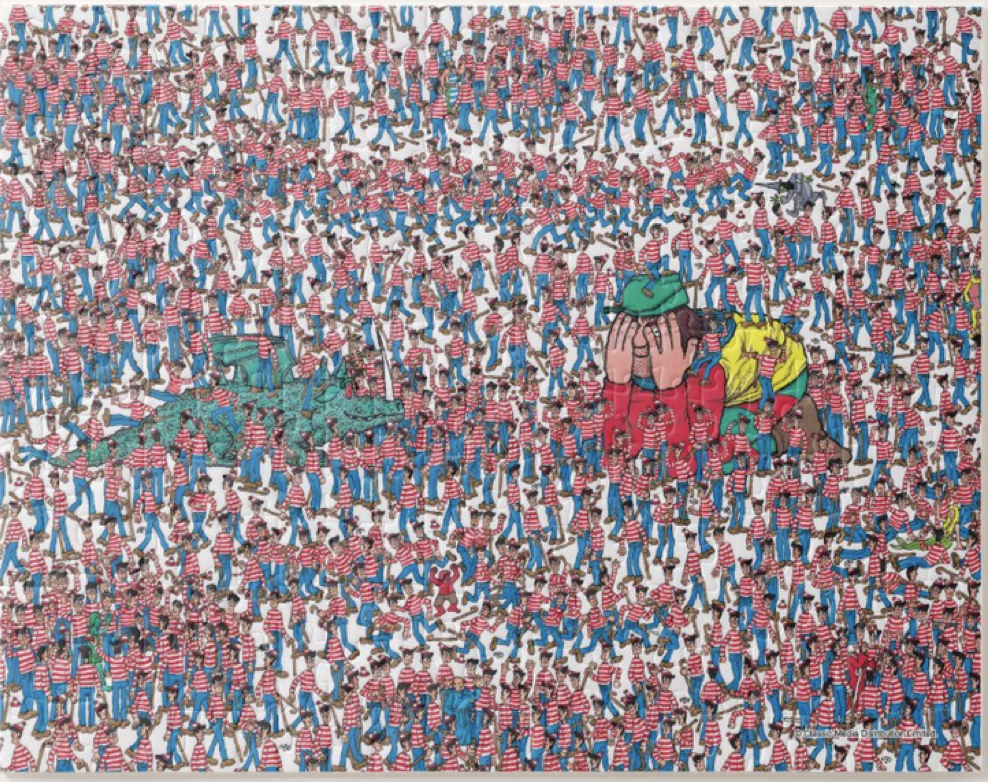
\includegraphics[keepaspectratio, width  = \textwidth]{img/waldo}\\
		\end{column}
		\end{columns}

\end{frame}
	
\begin{frame}


\centering \Large \textbf{Why do mutations have the potential to influence phenotypes?} \\

\begin{columns}
	\begin{column}{0.5\textwidth}
		\centering	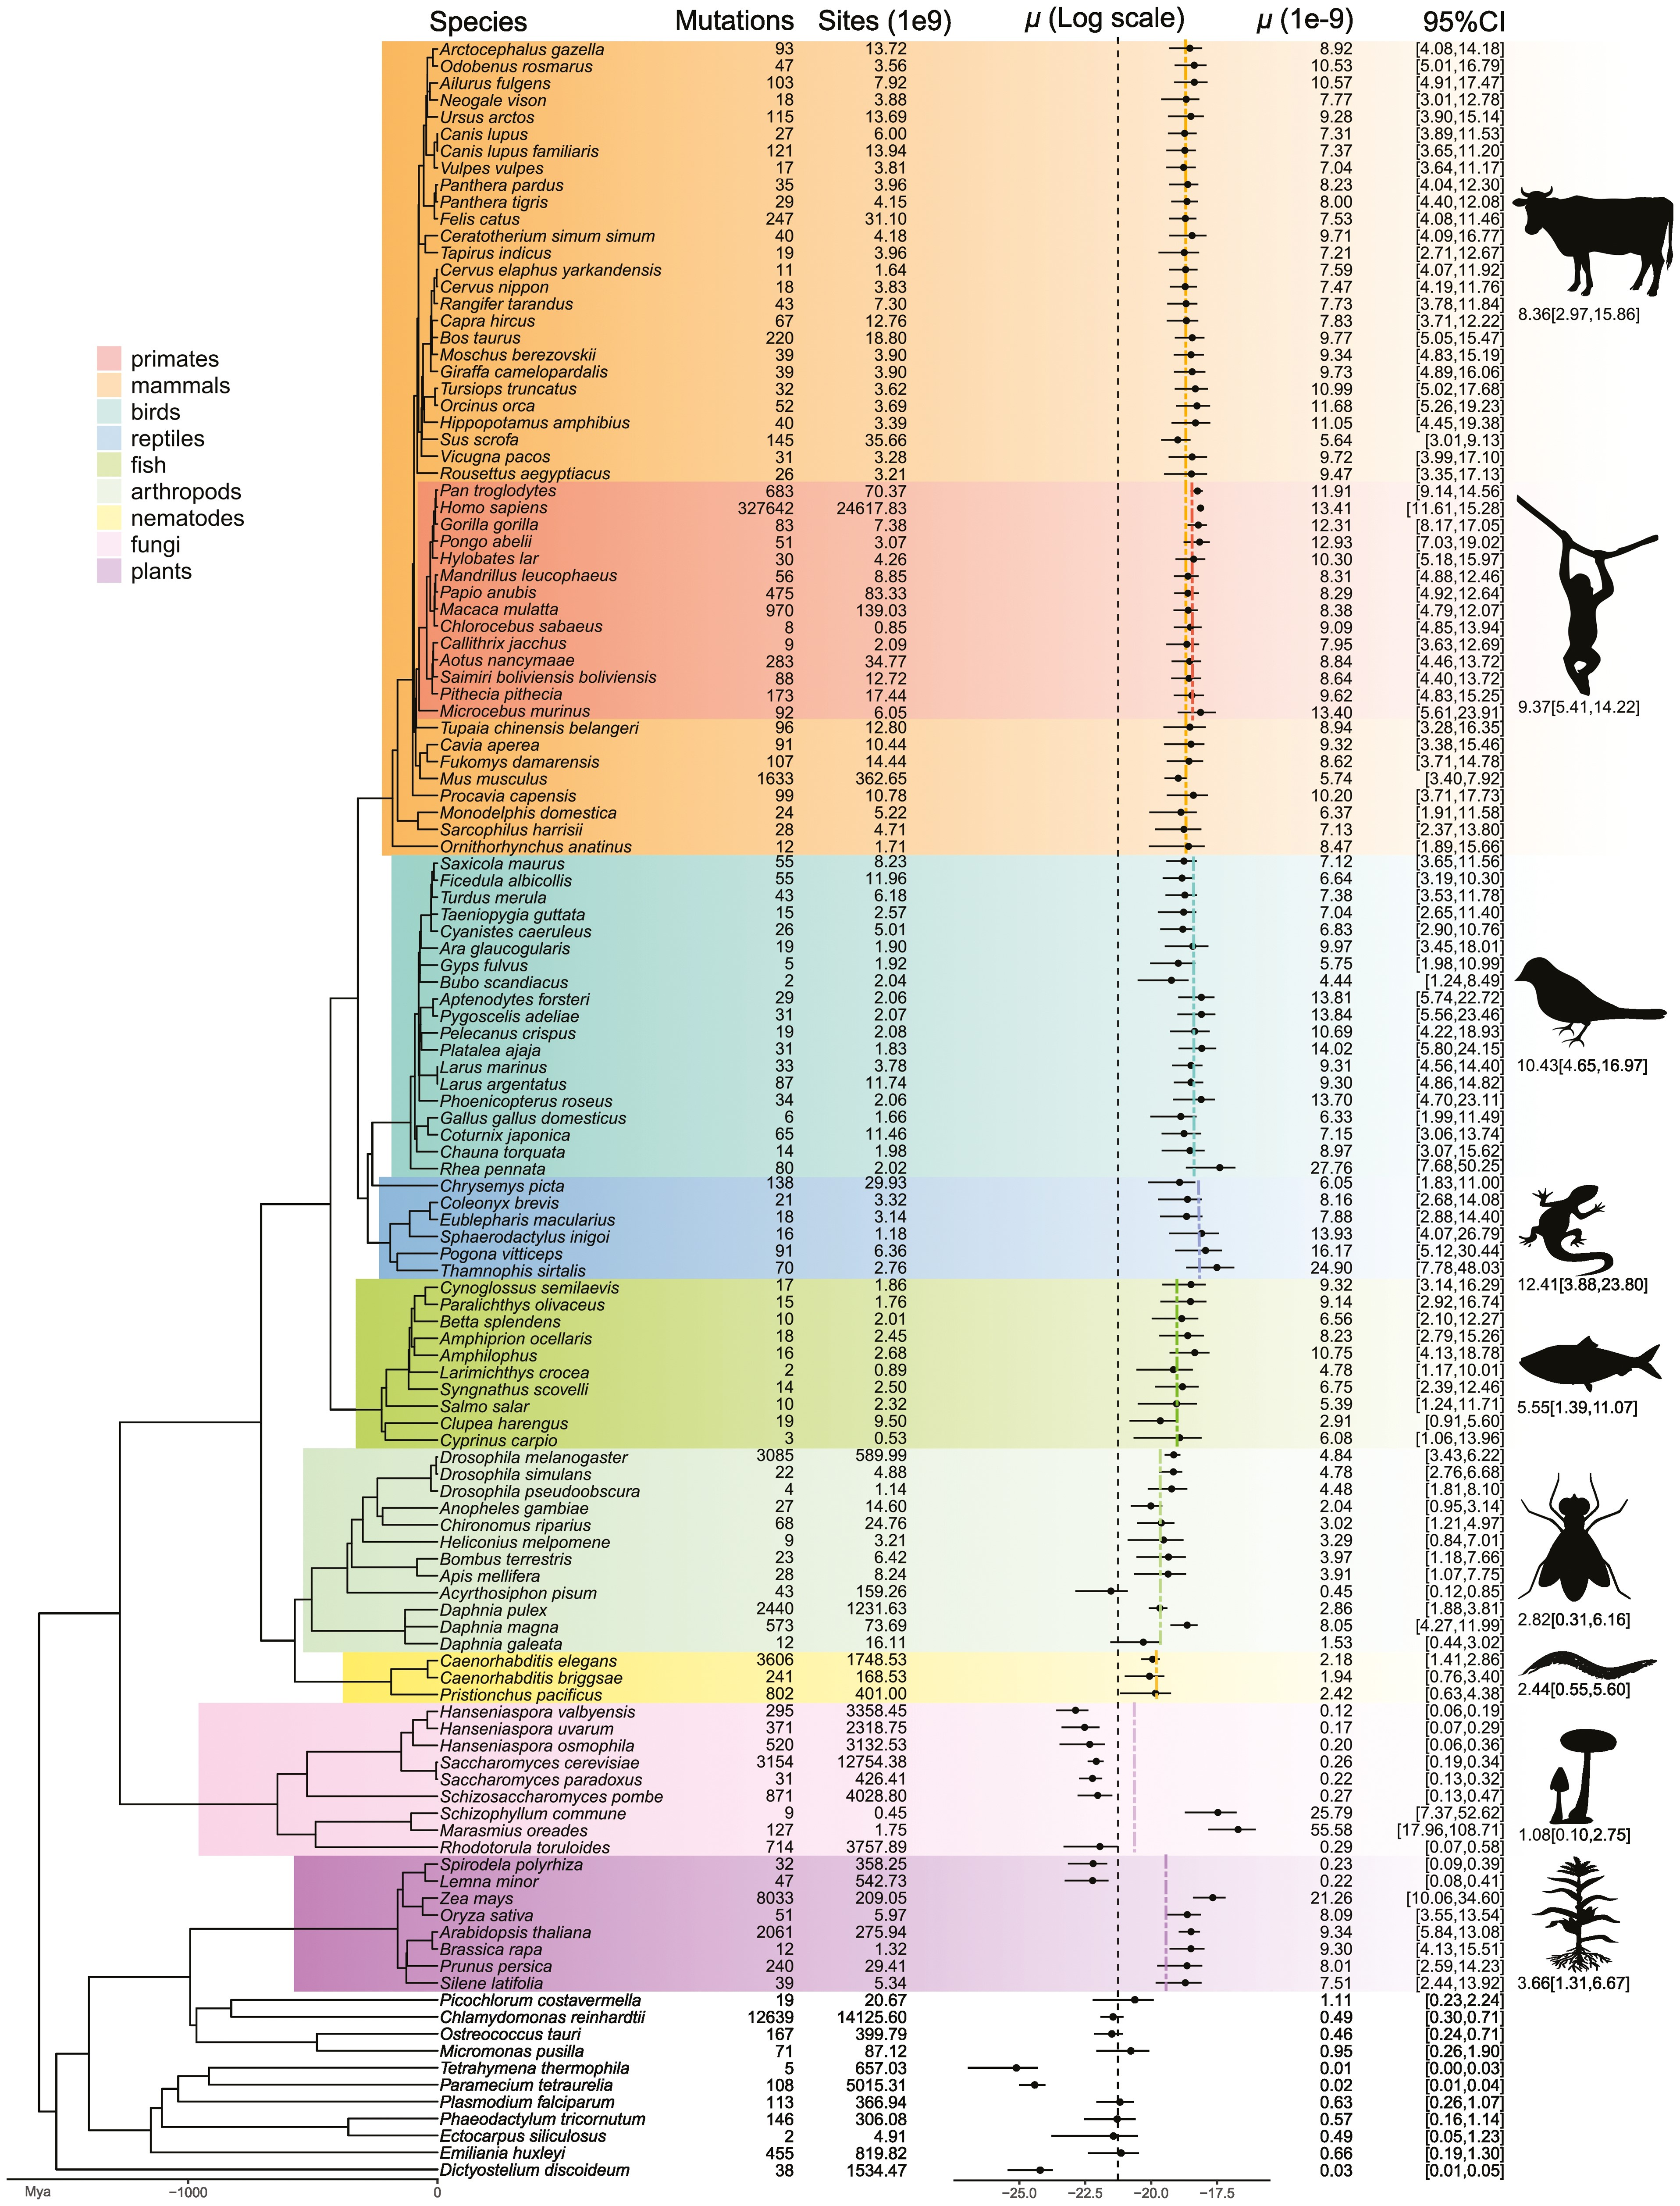
\includegraphics[keepaspectratio, width  = 0.8\textwidth]{img/mutationRates}\\
		\end{column}
	\begin{column}{0.5\textwidth}
		\centering	
\includegraphics[keepaspectratio, width  = \textwidth]{img/logan}\\
	\end{column}
	\end{columns}
\end{frame}
	
	

\begin{frame}

	
	
			The genome is the ``blueprint of life", so alterations to it can influence phenotypes\\
			
\vspace{15pt}			
		
			\centering	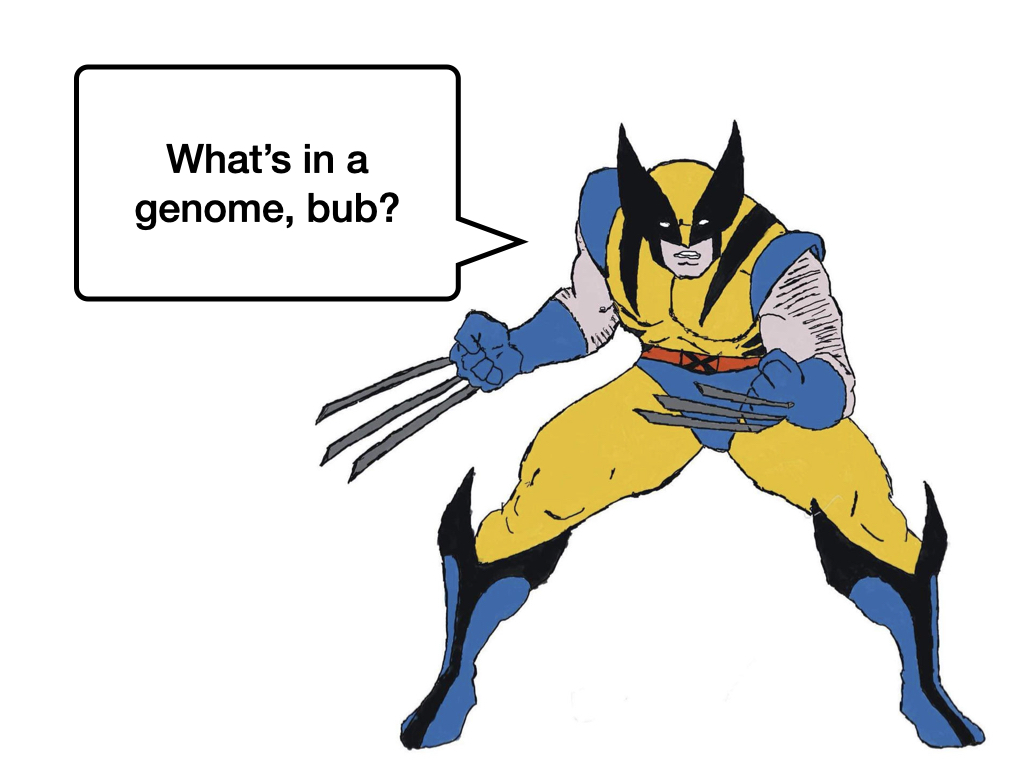
\includegraphics[keepaspectratio, width  = 0.6\textwidth]{img/logantalking}\\
	
\blfootnote{What is a phenotype? Any measurable characteristic of an individual. But remember that an individual's phenotype represents a combination of its environment and its genotype}
\end{frame}


\begin{frame}
	\frametitle{What's in a Genome?}
	
	
	\begin{columns}
		\begin{column}{0.33\textwidth}
			\centering	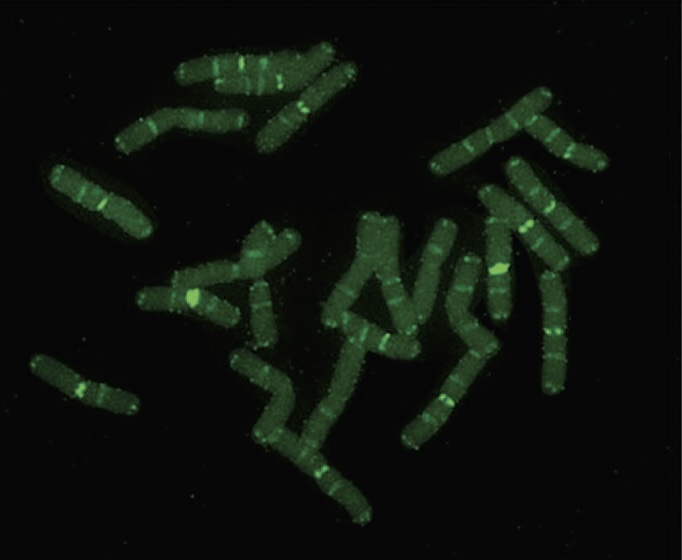
\includegraphics[keepaspectratio, width  = \textwidth]{img/loblollyChroms}\\ \pause
		\end{column}
		\begin{column}{0.33\textwidth}
			\centering	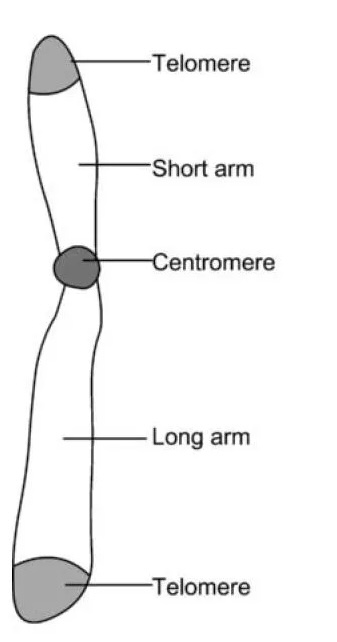
\includegraphics[keepaspectratio, width  = \textwidth]{img/chromosomeDiagram}\\ \pause
		\end{column}
		\begin{column}{0.33\textwidth}
			\centering	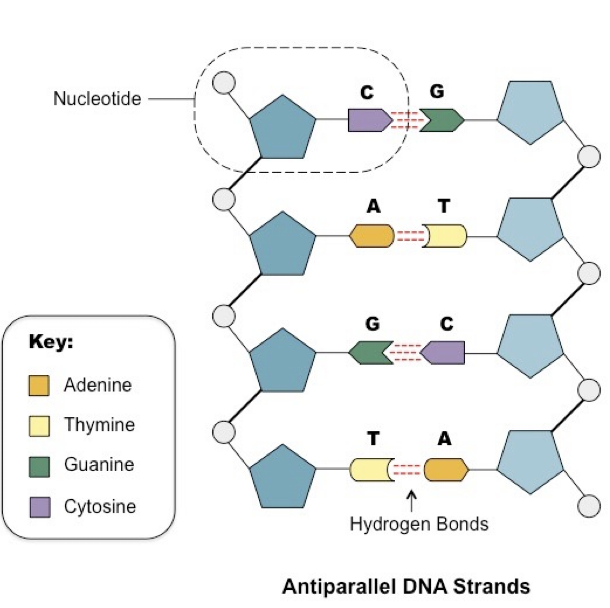
\includegraphics[keepaspectratio, width  = \textwidth]{img/DNA_cartoon}\\ 
	\end{column}
	\end{columns}
	
\centering	\Large But what does the DNA actually do?
\end{frame}



\begin{frame}
	\frametitle{Central Dogma of Molecular Biology}
	
	
	\centering	\Large \textit{``DNA makes RNA, and RNA makes protein"} \blfootnote{Francis Crick 1957}
	
				\centering	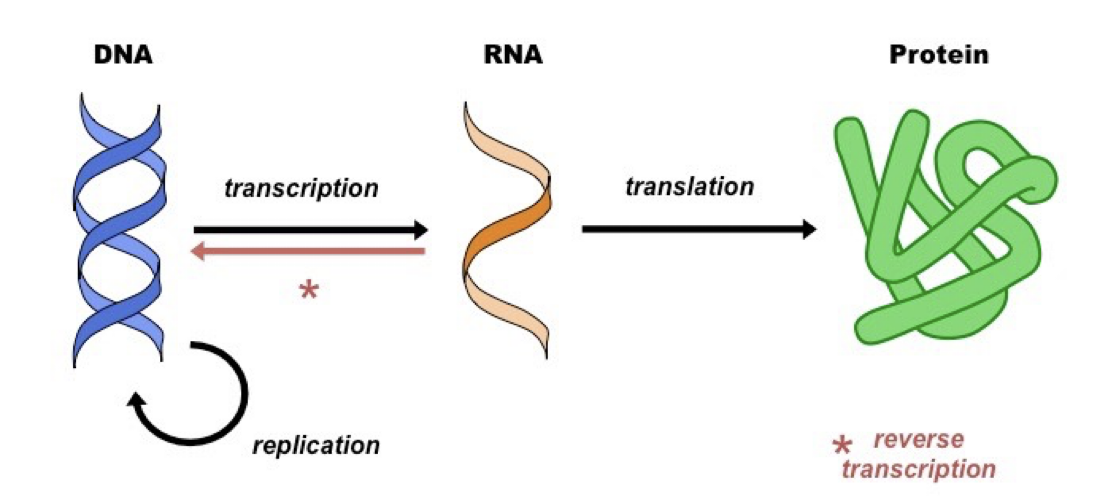
\includegraphics[keepaspectratio, width  = \textwidth]{img/dogma}\\ 
	
	\scriptsize \centering	It means that there is a one-way flow of information \\(\textit{But exceptions abound!})
	
\end{frame}



\begin{frame}
	\frametitle{Genes}
		
	\begin{columns}
		\begin{column}{0.5\textwidth}
		\begin{itemize}
			
			\item A \textbf{gene} is a section of DNA that controls a certain trait by encoding \textbf{proteins}
			\vspace{5pt}
			\item \textbf{Proteins/enzymes} do much of the work in the cell and the body 
			\vspace{5pt}
		
					\begin{itemize}
						\scriptsize
						\item[--] \textbf{Enzymes} are proteins that catalyze chemical reactions
						\item[--] Some proteins give cells their shape and structure an others carry our processes like energy conversion and phtosynthesis.
						\end{itemize}
		\end{itemize}

		\end{column}
		\begin{column}{0.5\textwidth}
			\centering	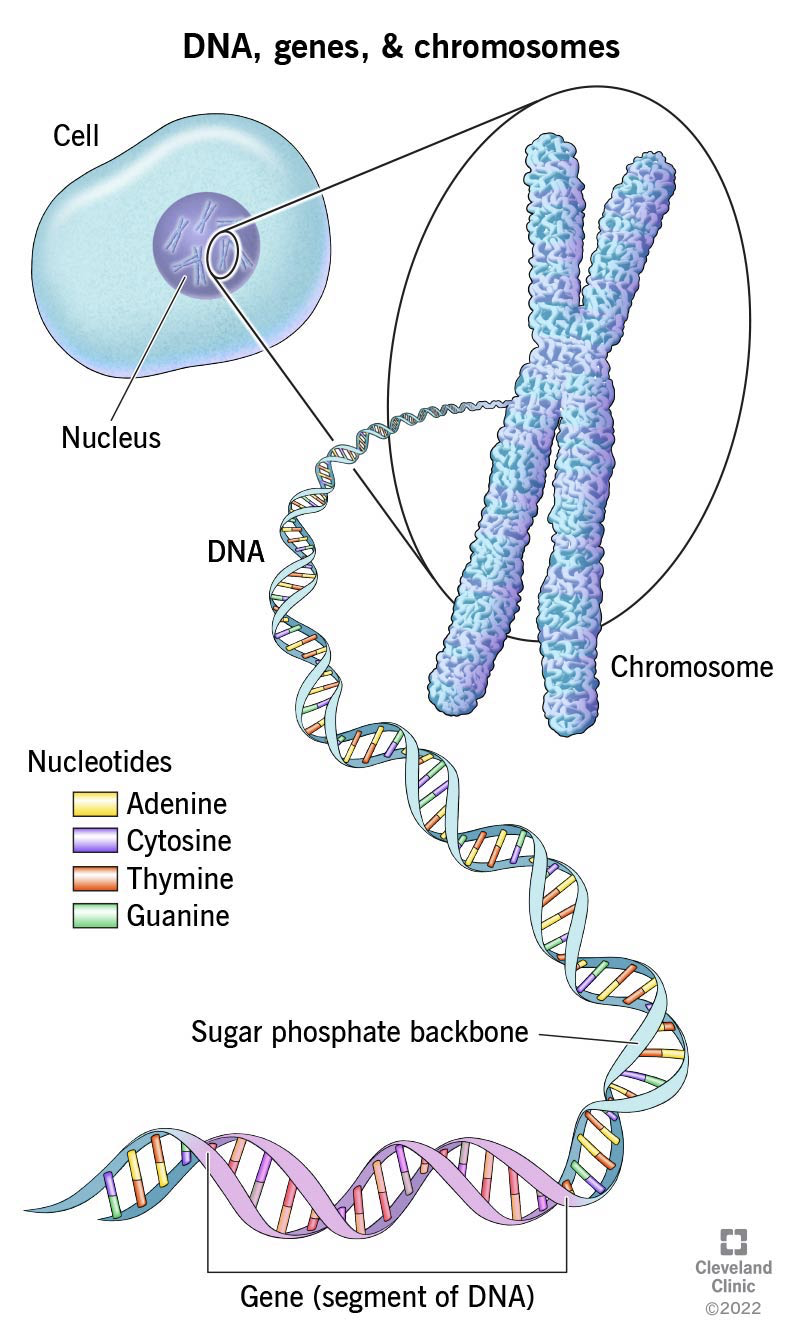
\includegraphics[keepaspectratio, width  = 0.9\textwidth]{img/geneOnDNA}\\
		\end{column}
	\end{columns}
	
\end{frame}


\begin{frame}
	\frametitle{Genes - Transcription and Translation}
	
	
	
	\begin{columns}
		\begin{column}{0.5\textwidth}
			\begin{itemize}
				\scriptsize
				\item Genes are expressed through the processes of \textbf{transcription} and \textbf{translation}
				\vspace{5pt}
				\item In \textbf{transcription}, DNA is used to produce a single stranded m(essenger) RNA molecule (note the pre-mRNA)
				\vspace{5pt}
				\item In translation, the specific set of nucleotides in the mRNA are used to build polypeptides (i.e. protein) 
			\end{itemize}
			
		\end{column}
		\begin{column}{0.5\textwidth}
			\centering	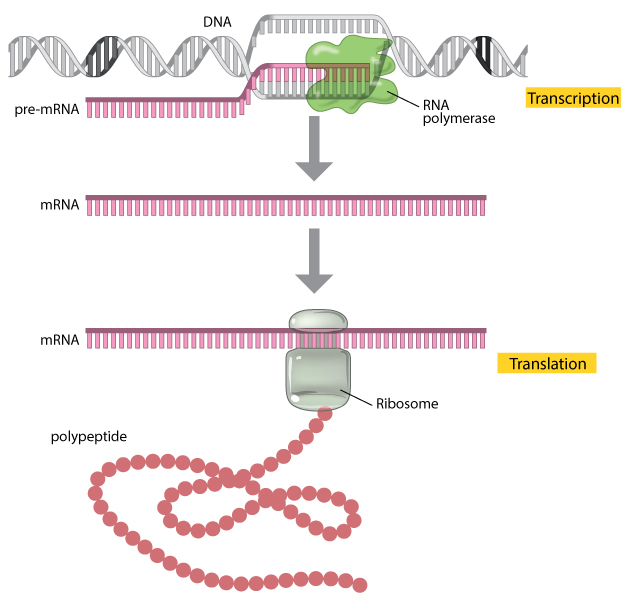
\includegraphics[keepaspectratio, width  = \textwidth]{img/dna2rna2protein}\\
		\end{column}
	\end{columns}
	
	\blfootnote{See \url{https://www.nature.com/scitable/topicpage/translation-dna-to-mrna-to-protein-393/} for a more complete primer}
\end{frame}



\begin{frame}
	\frametitle{RNA}
	
	\begin{itemize}
		\item Ribonucleic acid (RNA) is present in all cells
		\item Structurally similar to DNA, but usually single stranded \blfootnote{The genomes of many viruses are encoded by double-stranded RNA (e.g. rotavirus)}
		
	\end{itemize}
			\centering	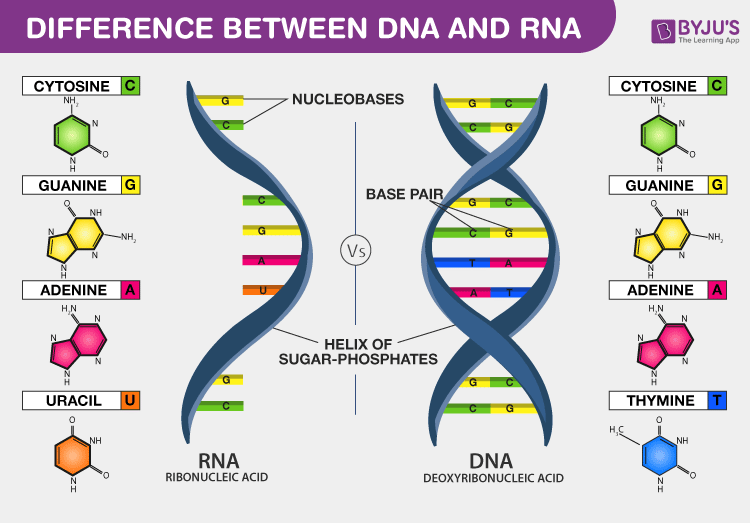
\includegraphics[keepaspectratio, width  = 0.8\textwidth]{img/rna_v_dna}\\
	
	
\end{frame}

\begin{frame}
\frametitle{Types of RNA}
	RNA plays a large number of roles in species' lifecycles, characterising these is an area of very active research\\
	
\vspace{20pt} 
	\scriptsize
	
	\begin{itemize}
\item mRNAs – messenger RNAs transcribed from genes
\item tRNAs – transfer RNAs for transferring amino acids
\item rRNAs – ribosome RNA involved in protein synthesizing (most abundant)
\item ncRNAs – non-coding RNA
\item lncRNAs – long non-coding RNAs ($>$100 base) seem to be involved in more or less everything!
\item miRNAs – microRNAs (21-23 bases) involved in mRNA silencing (gene regulation) 
\item piRNAs - Various roles including suppression of transposable elements
\end{itemize}
\vspace{20pt}
\textbf{All RNAs are encoded by DNA, but not all DNA encodes RNA!
}\end{frame}



\begin{frame}
	\frametitle{Genes - Translation}
	
	
	
	\begin{columns}
		\begin{column}{0.5\textwidth}
			\begin{itemize}
				\scriptsize
				\item In translation, ribosomes are recuited to synthesize the polypeptide
				\vspace{5pt}
				\item The sequence of the mRNA serves as the template
				\vspace{5pt}
				\item t(ransfer)RNA matching both amino acids and the genetic code of the mRNA are recruited by the ribosome
				\vspace{10pt}
				\item Watch this video in your spare time if you want to see a visualisation: \url{ https://youtu.be/gG7uCskUOrA}
			\end{itemize}
			
		\end{column}
		\begin{column}{0.5\textwidth}
			\centering	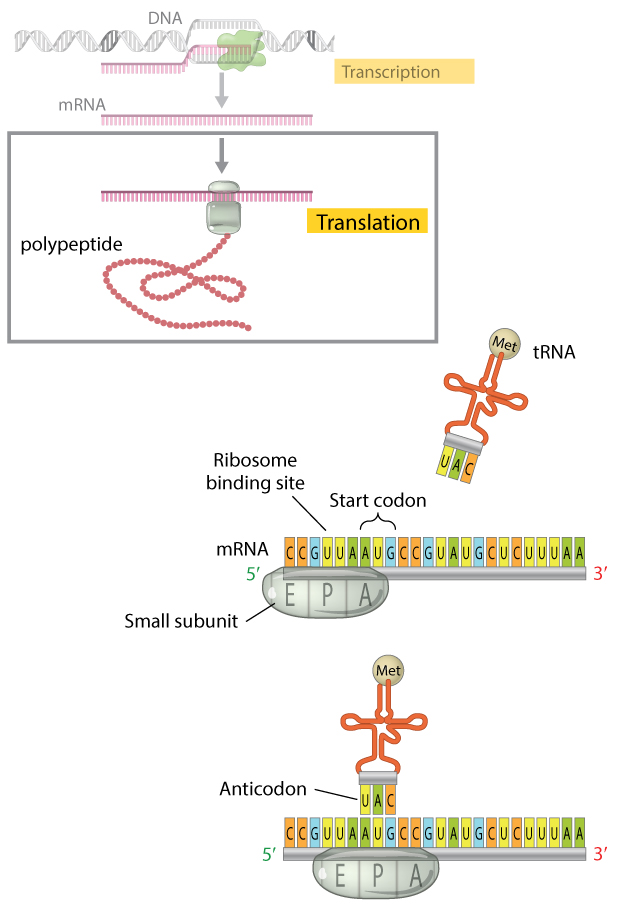
\includegraphics[keepaspectratio, width  = 0.9\textwidth]{img/translation}\\
		\end{column}
	\end{columns}
	
	\blfootnote{See \url{https://www.nature.com/scitable/topicpage/translation-dna-to-mrna-to-protein-393/} for a more complete primer}
\end{frame}


\begin{frame}
	\frametitle{Plant Cell}
	\centering	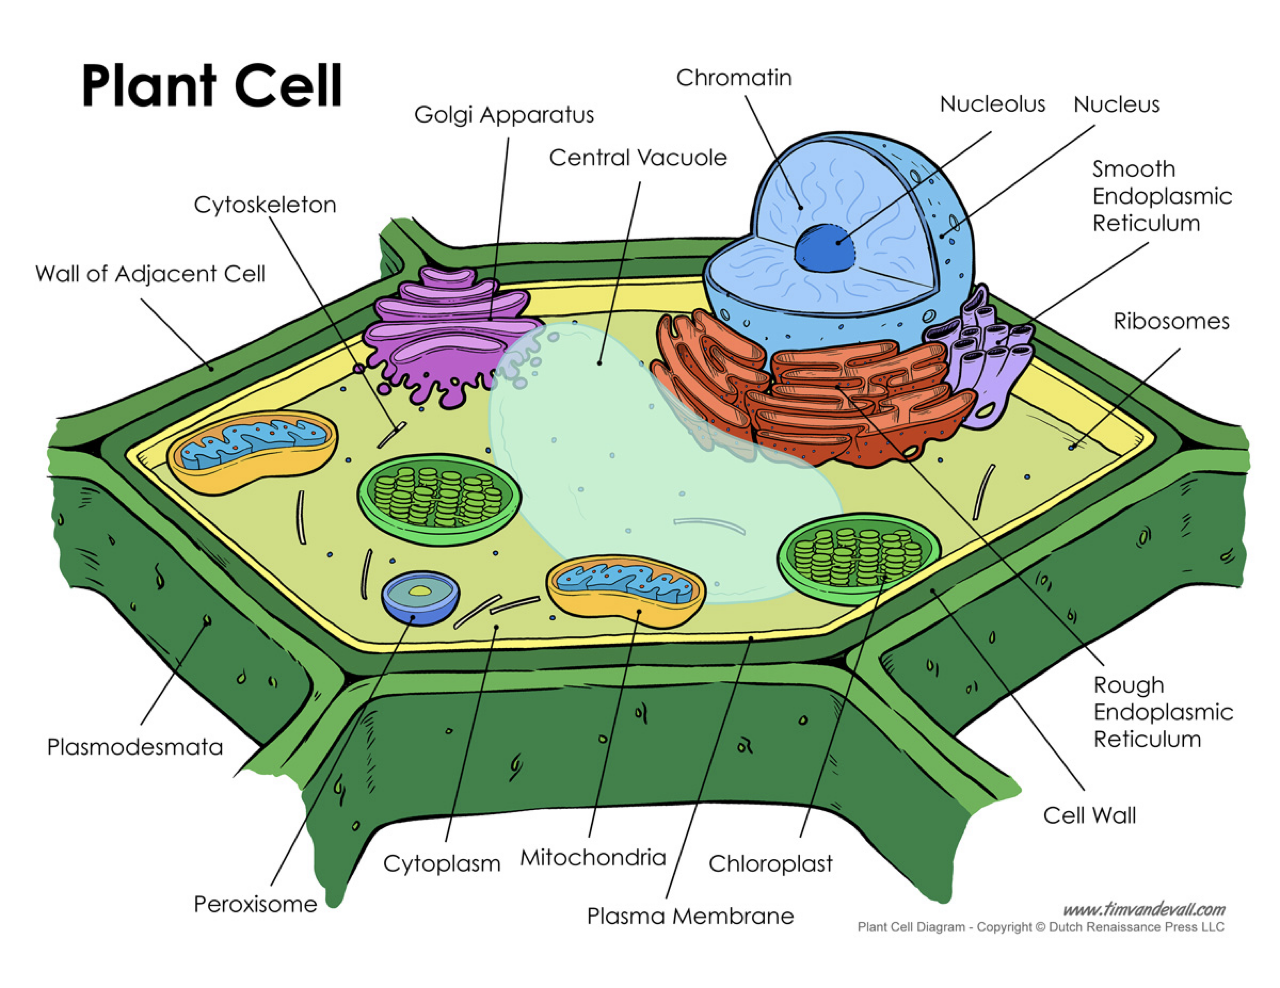
\includegraphics[keepaspectratio, width  =1\textwidth]{img/plantCell}\\
\end{frame}



\begin{frame}
	\frametitle{Genes - Translation and the Genetic Code}
	
	
	
	\begin{columns}
	
		\begin{column}{0.5\textwidth}
			\centering	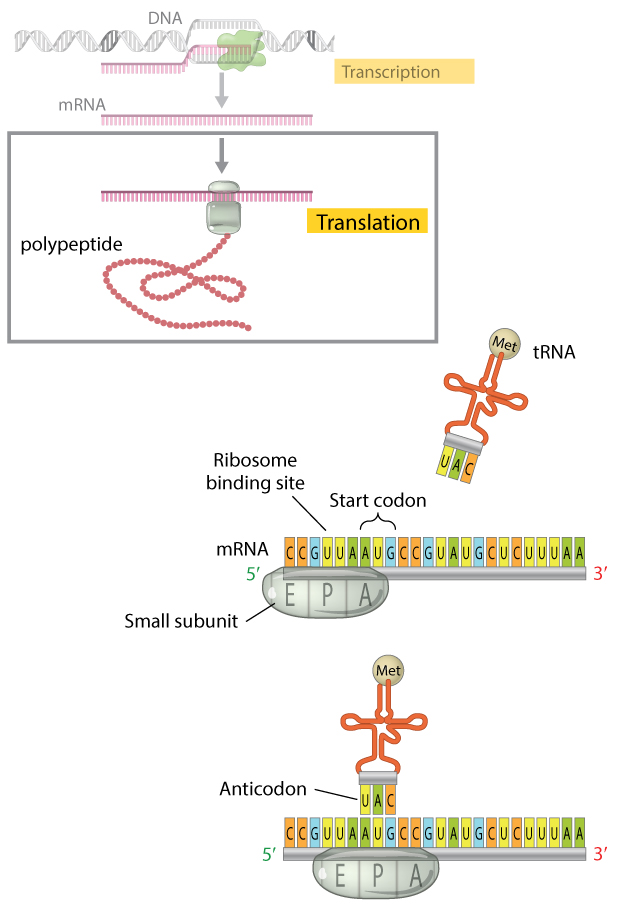
\includegraphics[keepaspectratio, width  = 0.9\textwidth]{img/translation}\\
		\end{column}
	\begin{column}{0.5\textwidth}
	
	\centering	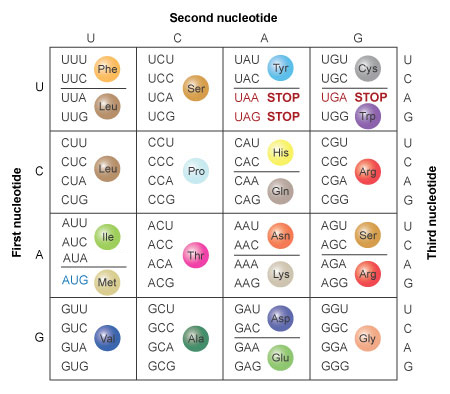
\includegraphics[keepaspectratio, width  = 0.9\textwidth]{img/geneticCode}\\
	\scriptsize			\begin{itemize}
		\item[--] Each possible set of three RNA nucleotides (i.e. codon) corresponds to a particular amino acid
		\item[--] Note the synonymous codons!
		\item[--] Codons are written from 5` to 3`				
		\item[--] AUG (i.e. Methionine) is the start codon
	\end{itemize}			
	\end{column}
	\end{columns}
	
	\blfootnote{See \url{https://www.nature.com/scitable/topicpage/translation-dna-to-mrna-to-protein-393/} for a more complete primer}
\end{frame}


\begin{frame}
	\frametitle{Gene Structure}
	
	\centering	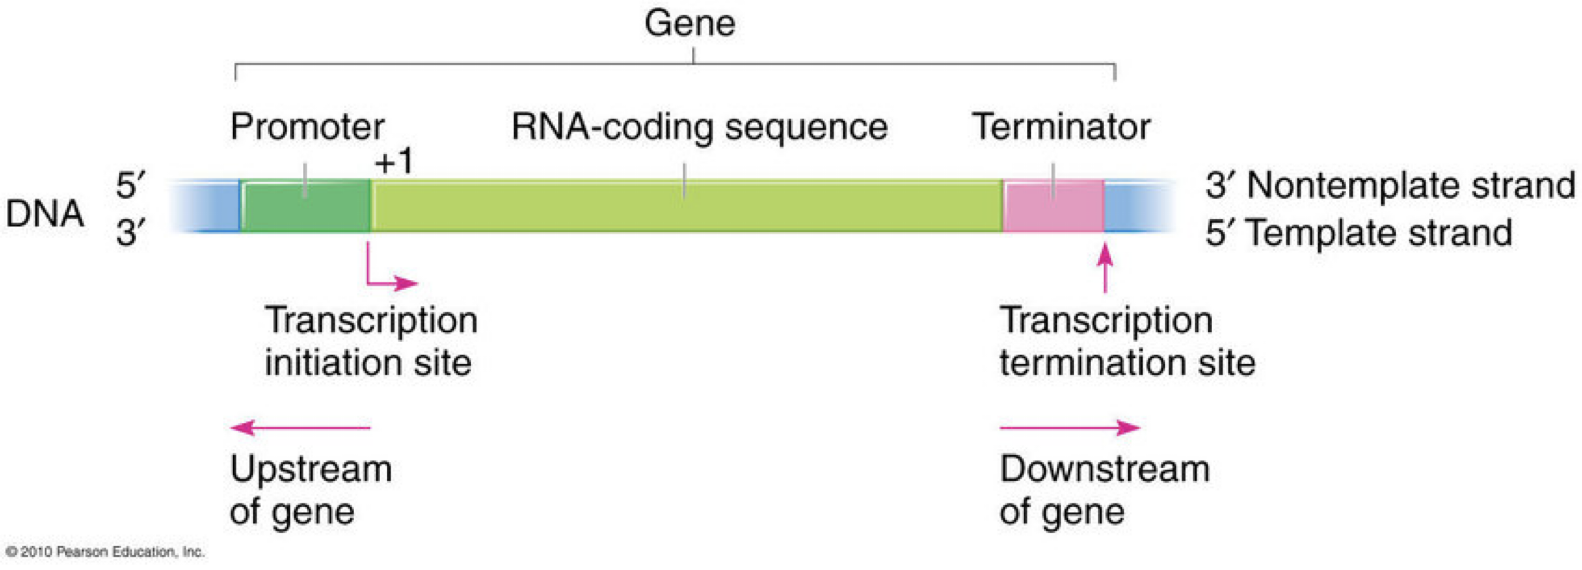
\includegraphics[keepaspectratio, width  = \textwidth]{img/geneStructure}\\ 

\end{frame}


\begin{frame}
	\frametitle{Gene Structure - Exons/Introns}
			\centering	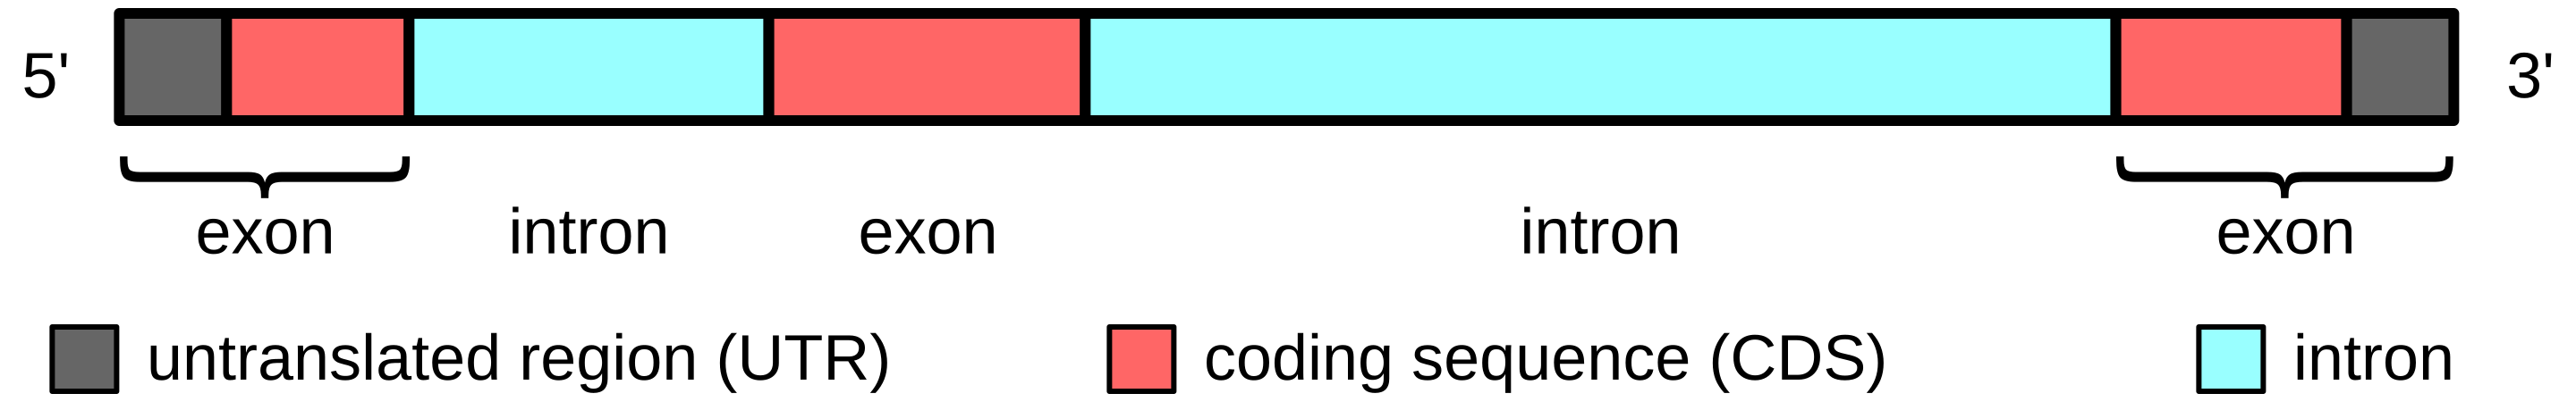
\includegraphics[keepaspectratio, width  = \textwidth]{img/geneStructureCartoon}\\ 
			
			\begin{itemize}
				\item \textbf{Exon} - DNA/RNA sequence that encodes the amino acid sequence
				\item \textbf{Intron} - Non-coding DNA/RNA interspersed between exons in most genes
				\item \textbf{UTR} - Untranslated regions of the mRNA that allow for binding of the ribosome (5') and for translation termination (3')
			\end{itemize}
\end{frame}


\begin{frame}
	\frametitle{Douglas-fir Genes}
	\scriptsize
	\begin{columns}
	\begin{column}{0.7\textwidth}
	\begin{tabular}{r|c}
		Total genes	& 51,419\\
		Average gene length (bp) & 17,967.11\\
		Median gene length (bp) & 1,962 \\
		Multiexonics & 41,595\\
		Monoexonics & 9,824\\
		Longest intron (kb) & 778,429\\
		Average number of exons per multiexonic gene& 4.73\\
		
	\end{tabular}		
\end{column}
\begin{column}{0.3\textwidth}
			\centering	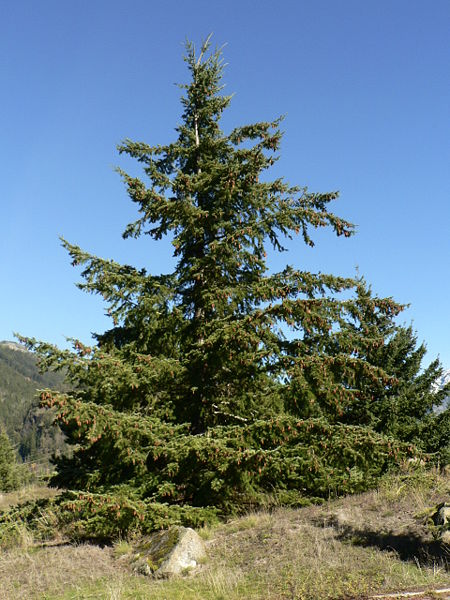
\includegraphics[keepaspectratio, width  = \textwidth]{img/doug-fir}
\end{column}
\end{columns}

\pause 
\vspace{20pt}
Think about all the different tissue types, cell types and developmental steps that characterize a Doiuglas-fir throughout its life \\
\vspace{10pt}
\textbf{How does a set of $51,419$ proteins do all of those things?}

	\blfootnote{Data from: Velasco et al 2023 - \textit{G3}}
\end{frame}





\begin{frame}
	
	\Huge
	Questions? \\ \pause
	Let's take a short break
	
\end{frame}


\begin{frame}
		\centering	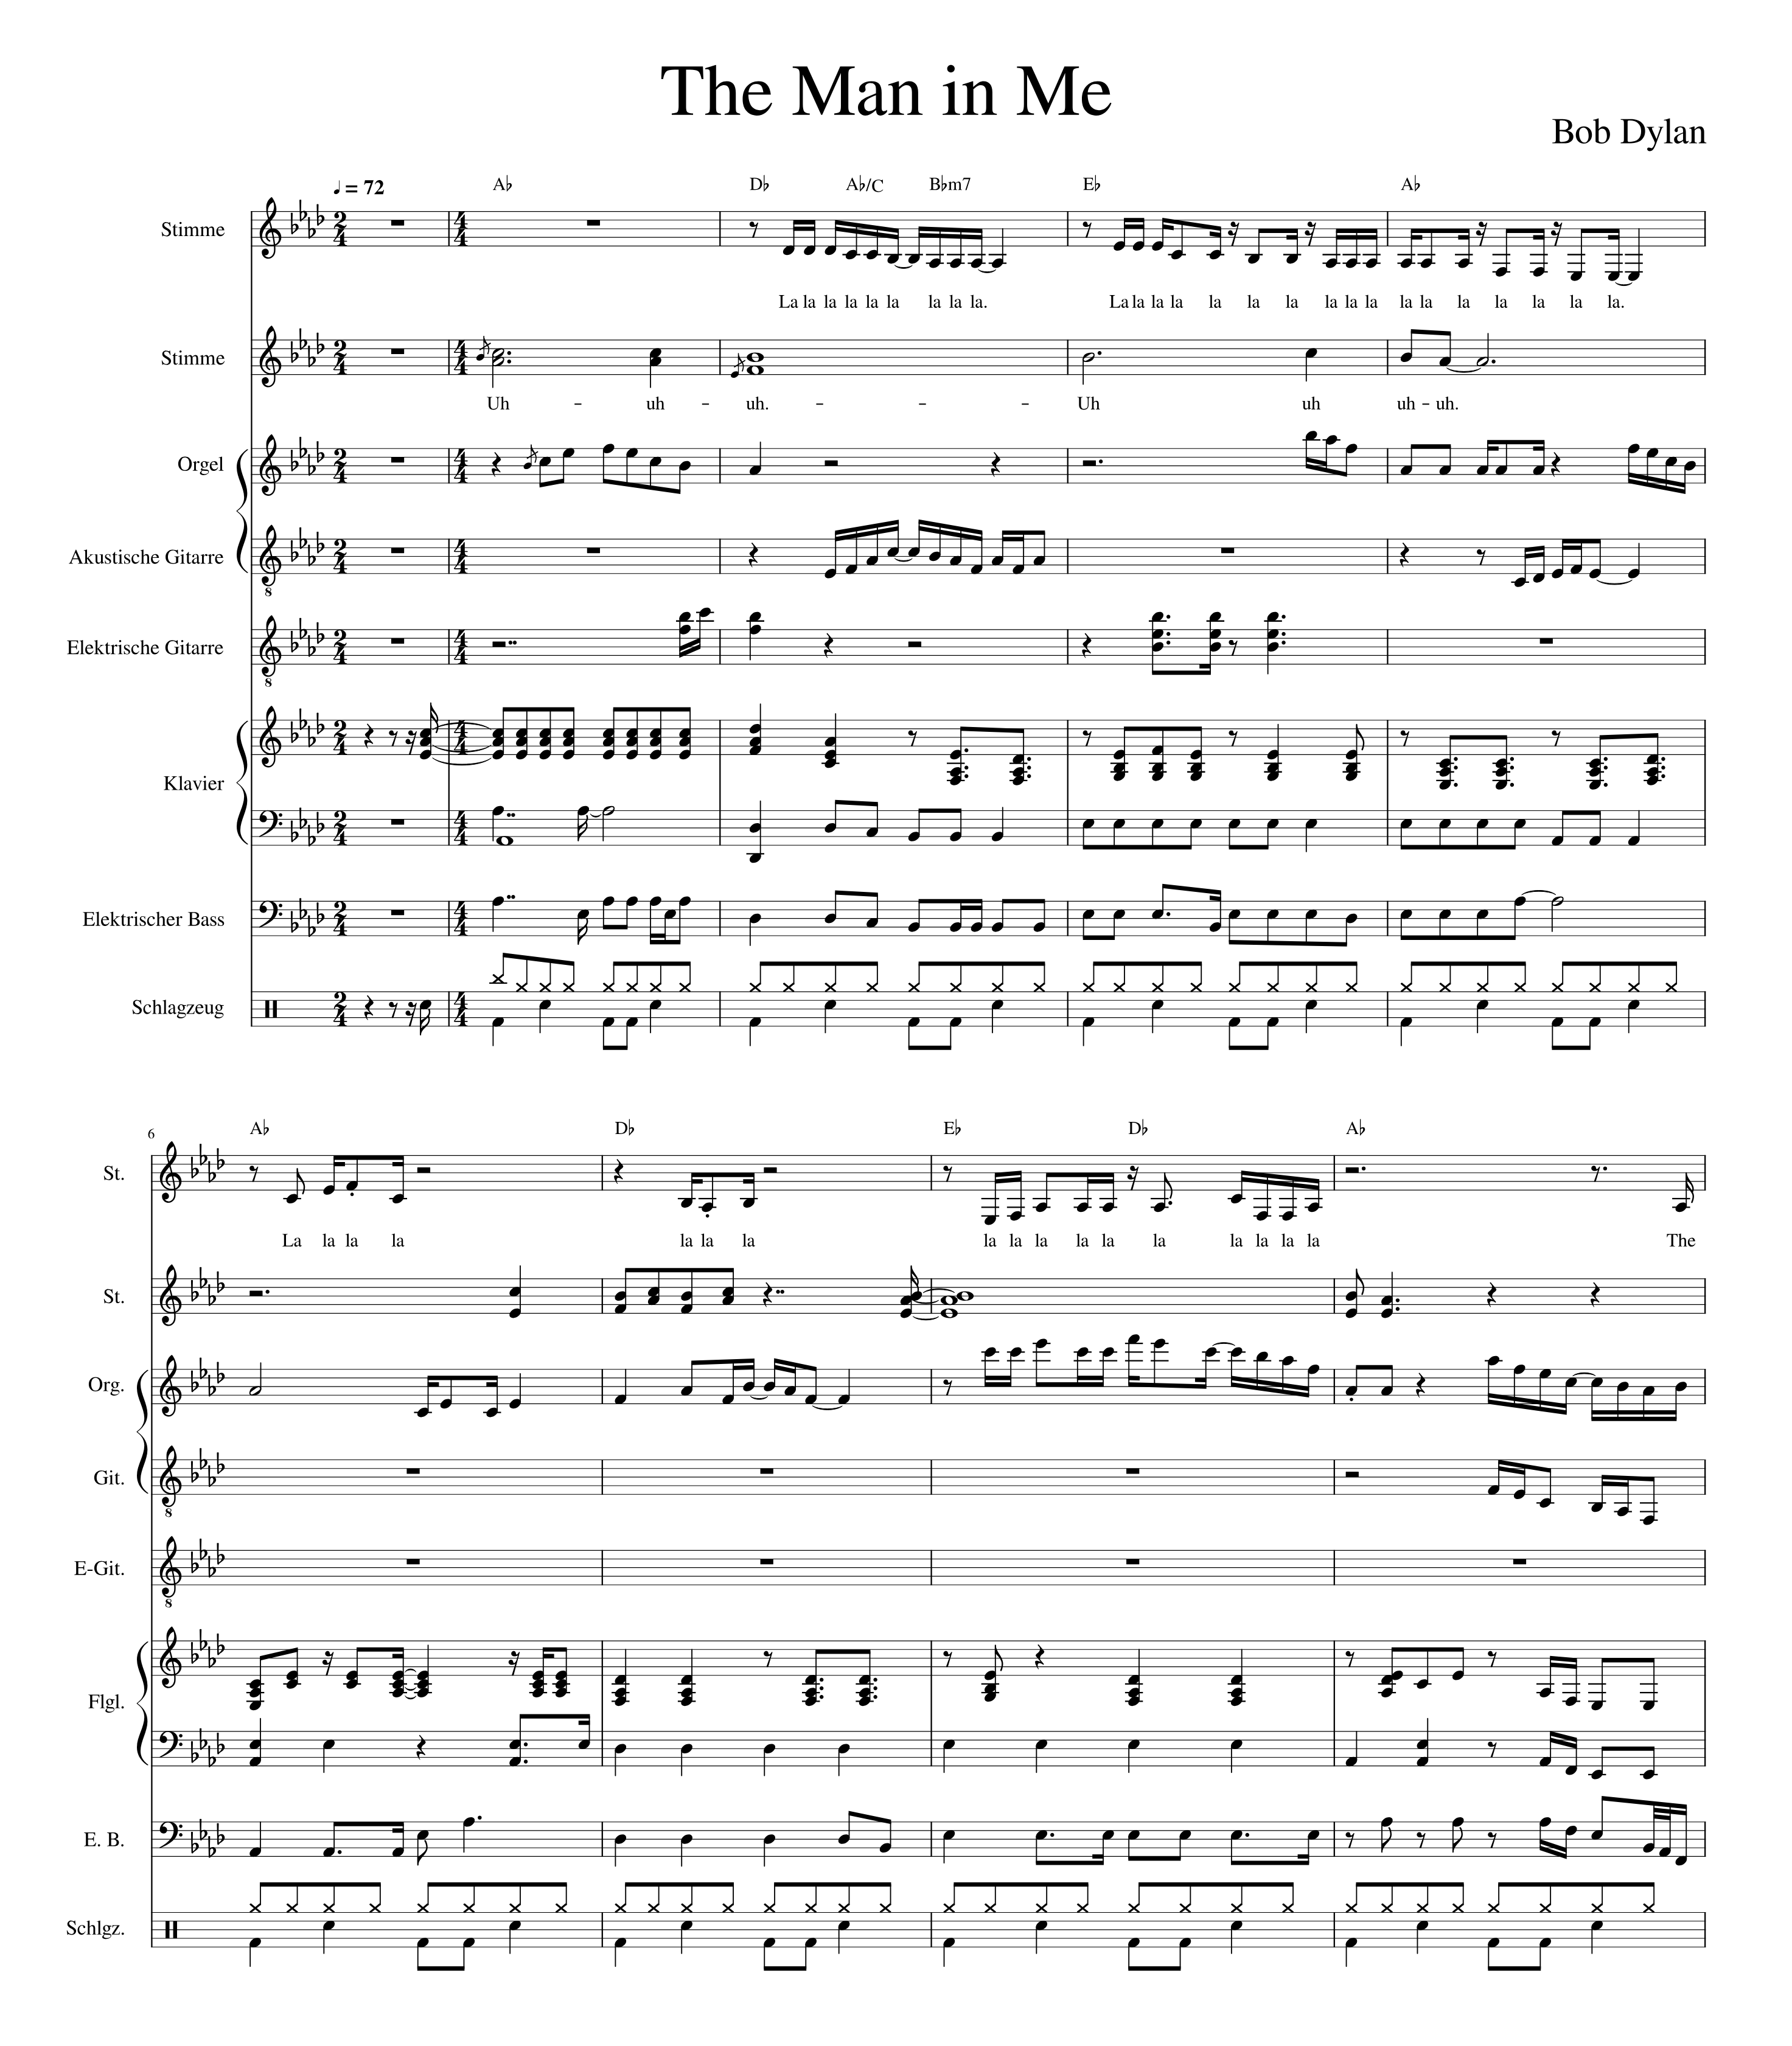
\includegraphics[keepaspectratio, width  = 0.7\textwidth]{img/bobd}\\ \pause
If genes are the orchestra, gene expression is the music
\end{frame}


\begin{frame}
	\frametitle{Components of Gene Regulation}
	\begin{columns}
		
		\begin{column}{0.5\textwidth}
			\scriptsize
			\begin{itemize}
				
				\item[] Chromatin accessibility
				\item[] Transcription
				\begin{itemize}
					\item[] Promoters, enhancers, silencers
				\end{itemize}
				\item[] RNA processing
				\item[] RNA stability
				\begin{itemize}
					\item[] The longer it stays, the greater chance of translating the protein
				\end{itemize}
				\item[] Translation
				\item[] Protein activity
			\end{itemize}
		\end{column}
		\begin{column}{0.5\textwidth}
			\centering	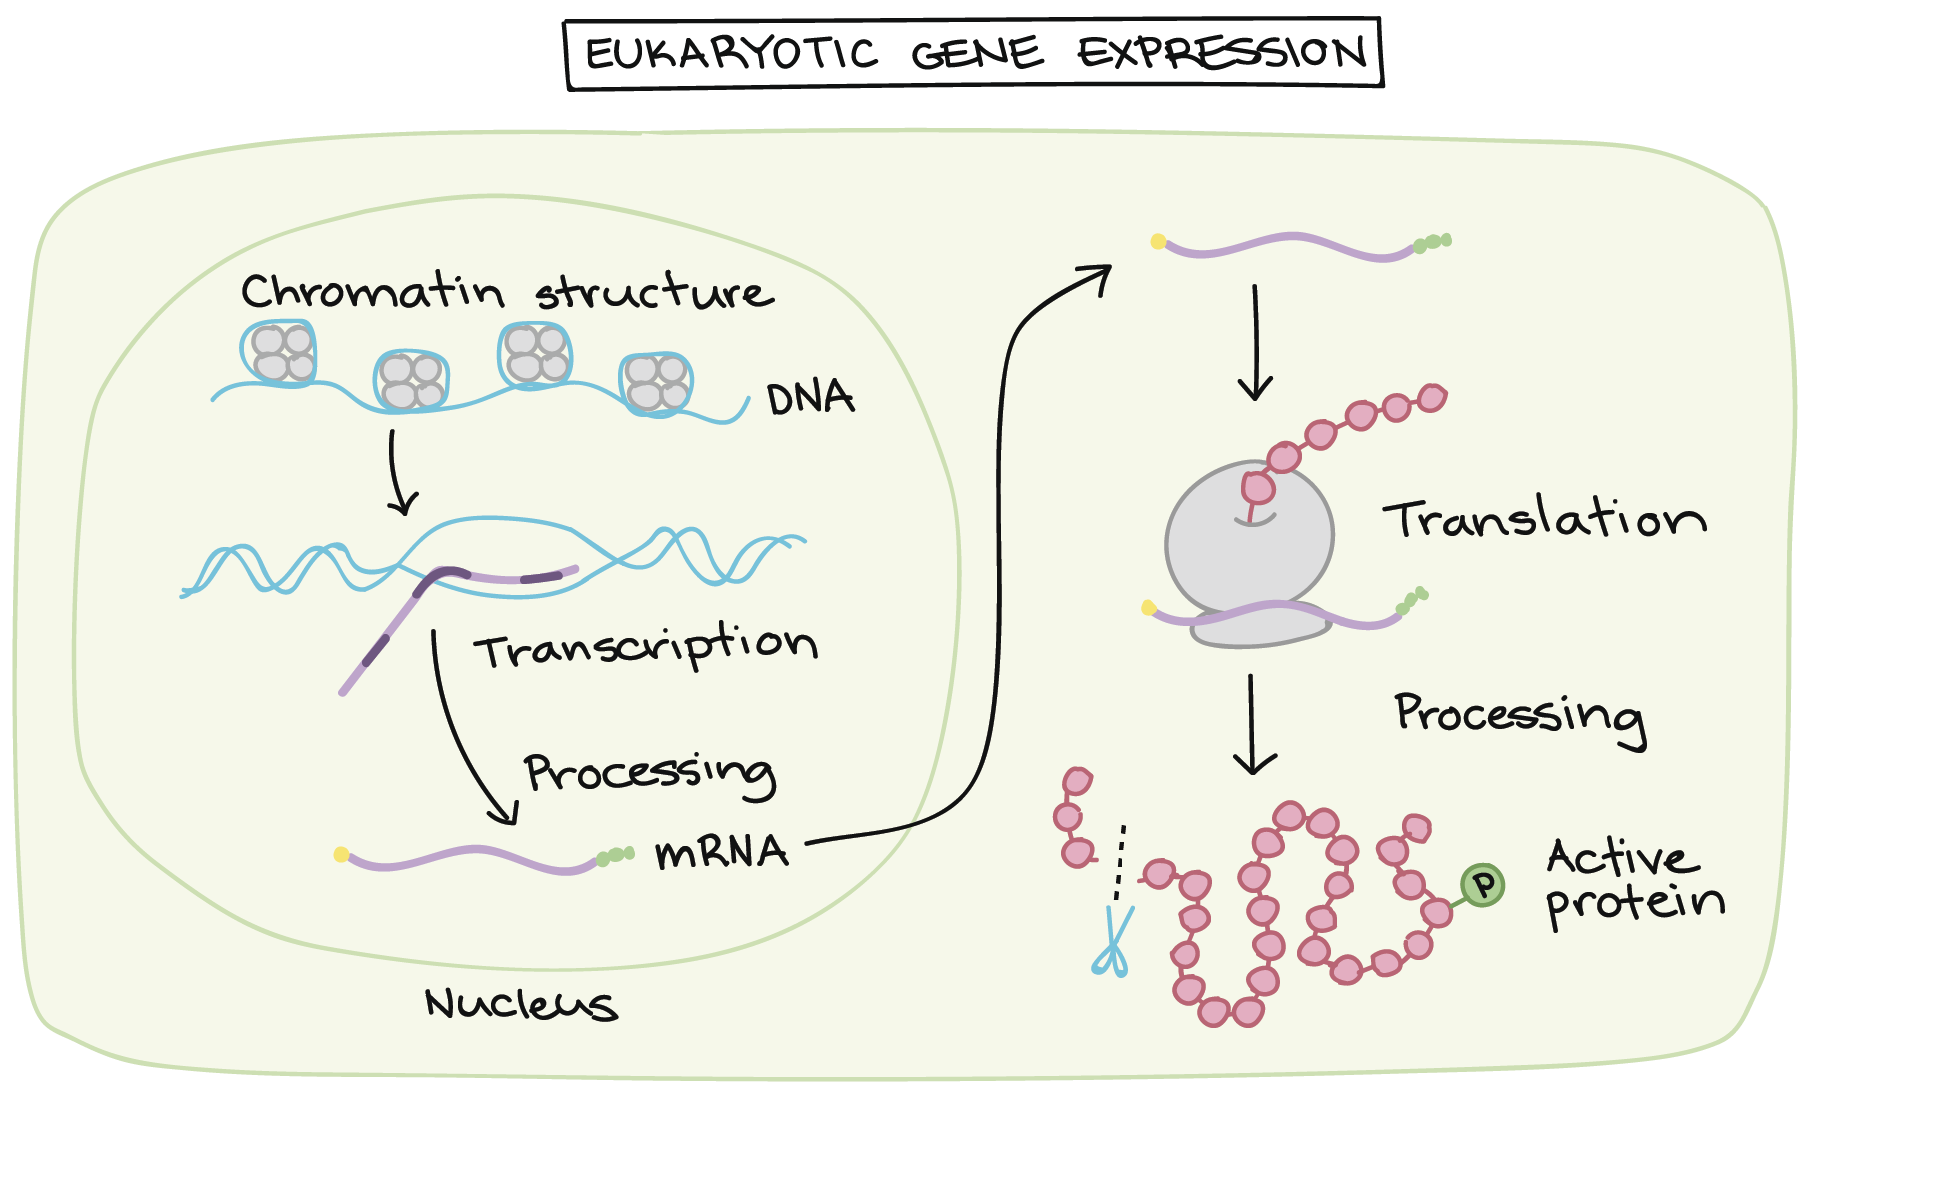
\includegraphics[keepaspectratio, width  = \textwidth]{img/geneExpressionCartoon}
		\end{column}
	\end{columns}	
	
\end{frame}

\begin{frame}
	\frametitle{Chromatin Accessibility}
				\centering	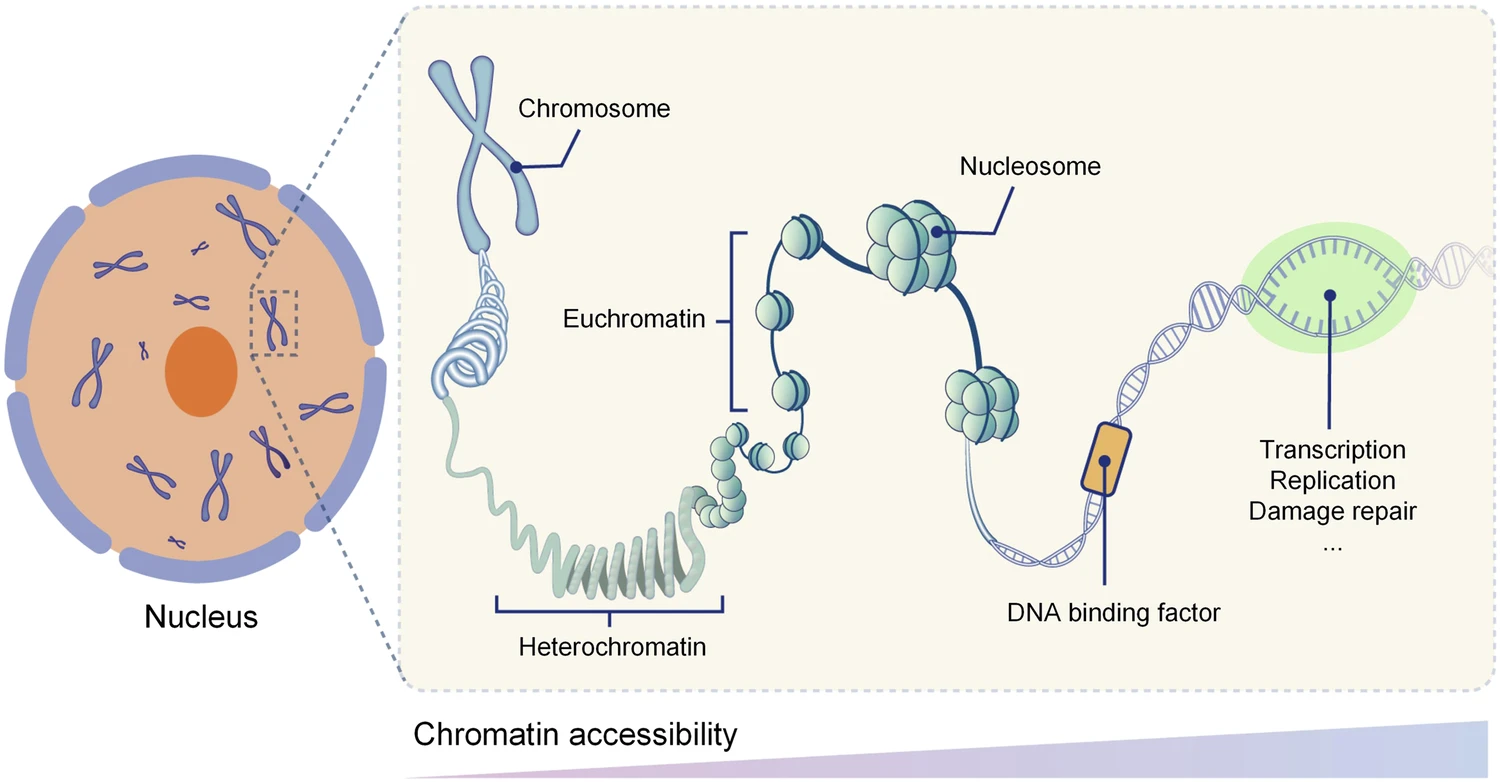
\includegraphics[keepaspectratio, width  = \textwidth]{img/chromatinAccessibilty}\\
				In order for transcription to occur, a gene needs to be located in accessible chromatin\\
				The dynamics of regions becoming more or less accessible is characteristic of eukaryotic organisms\\
				\blfootnote{Figure from: Chen et al 2024 - Sign. Transd.}
				
			
\end{frame}


\begin{frame}
	\frametitle{Gene Regulation - Promoters and Enhancers }
	\begin{columns}
		\begin{column}{0.5\textwidth}
			\centering	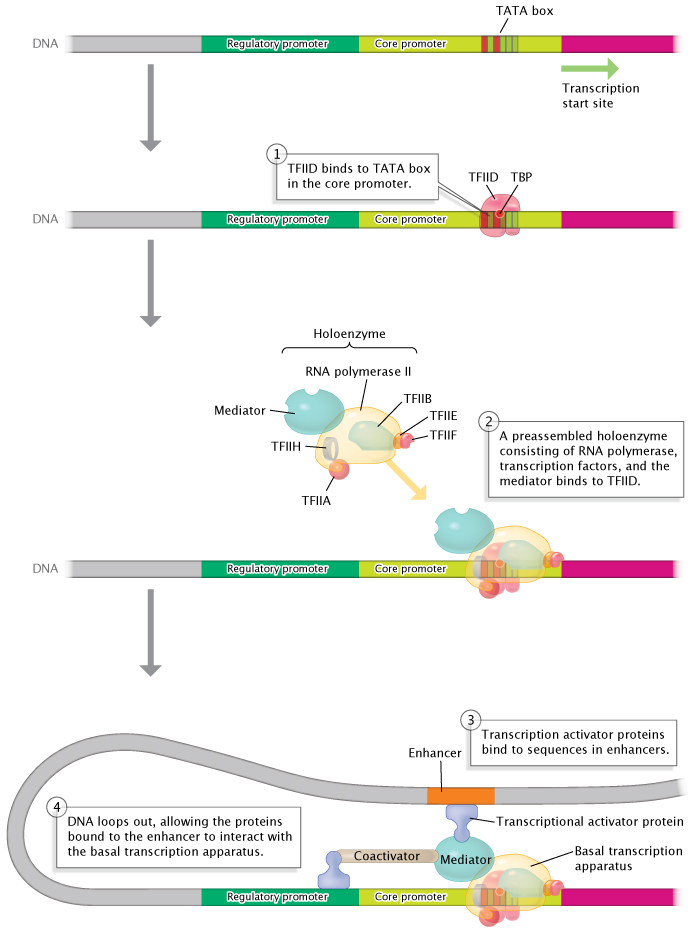
\includegraphics[keepaspectratio, width  = 0.9\textwidth]{img/initiatingExpression}
		\end{column}
		\begin{column}{0.5\textwidth}
			\scriptsize
			\textbf{Promoters}
			\begin{itemize}
				\item 100-1000bp long, located just upstream of transcription start site
				\item TATA box usually located 5-bp upstream of transcription start site
				\item Contains specific sequences that bind proteins to initiate transcription \pause
			\end{itemize}
			\textbf{Enhancers}
			\begin{itemize}
				\item Potentially located far away from transcription start site
				\item Contains specific sequences that bind proteins to amplify or make transcription more likely
			\end{itemize} \pause
			\textbf{Silencers \& Insulators}
			\begin{itemize}
				\item Other binding sites that can influence or prevent transcription at particular sites in the genome
				\item Contains specific sequences that bind proteins and influence transcription
			\end{itemize}
		\end{column}
	\end{columns}	
	\blfootnote{See a more detailed primer here: \url{https://www.nature.com/scitable/topicpage/what-is-a-gene-colinearity-and-transcription-430}}
	
\end{frame}


\begin{frame}
	\frametitle{Gene Structure - Exons/Introns}
	\centering	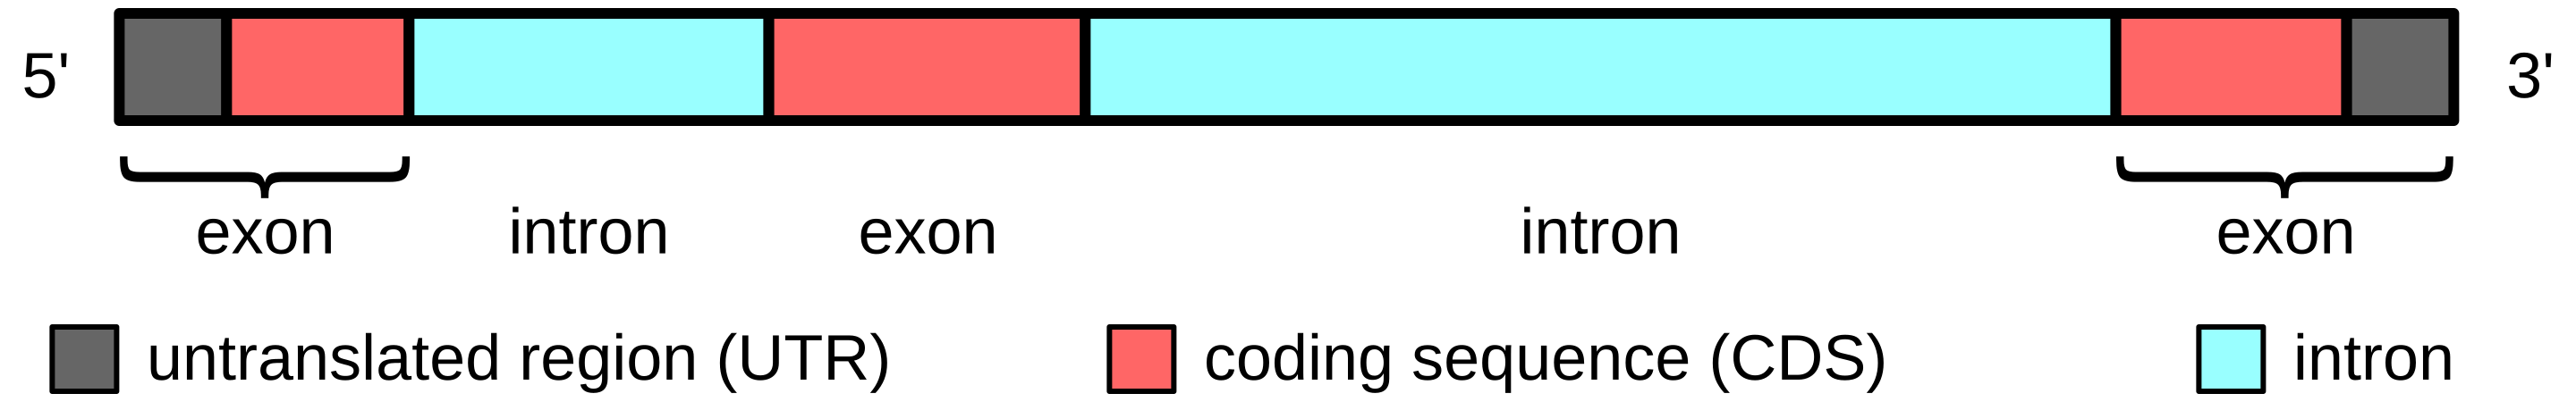
\includegraphics[keepaspectratio, width  = \textwidth]{img/geneStructureCartoon}\\ 
	\vspace{15pt}

	
	\begin{itemize}
		\item \textbf{Exon} - DNA/RNA sequence that encodes the amino acid sequence
		\item \textbf{Intron} - Non-coding DNA/RNA interspersed between exons in most genes
		\item \textbf{UTR} - Untranslated regions of the mRNA that allow for binding of the ribosome (5') and for translation termination (3')
	\end{itemize}
\end{frame}

\begin{frame}
	\frametitle{Gene Structure - Alternative Splicing}
	
\scriptsize
	A multi-exonic gene is capable of making many different isoforms (or splice variants) that potentially encode different protein products\\
	\centering	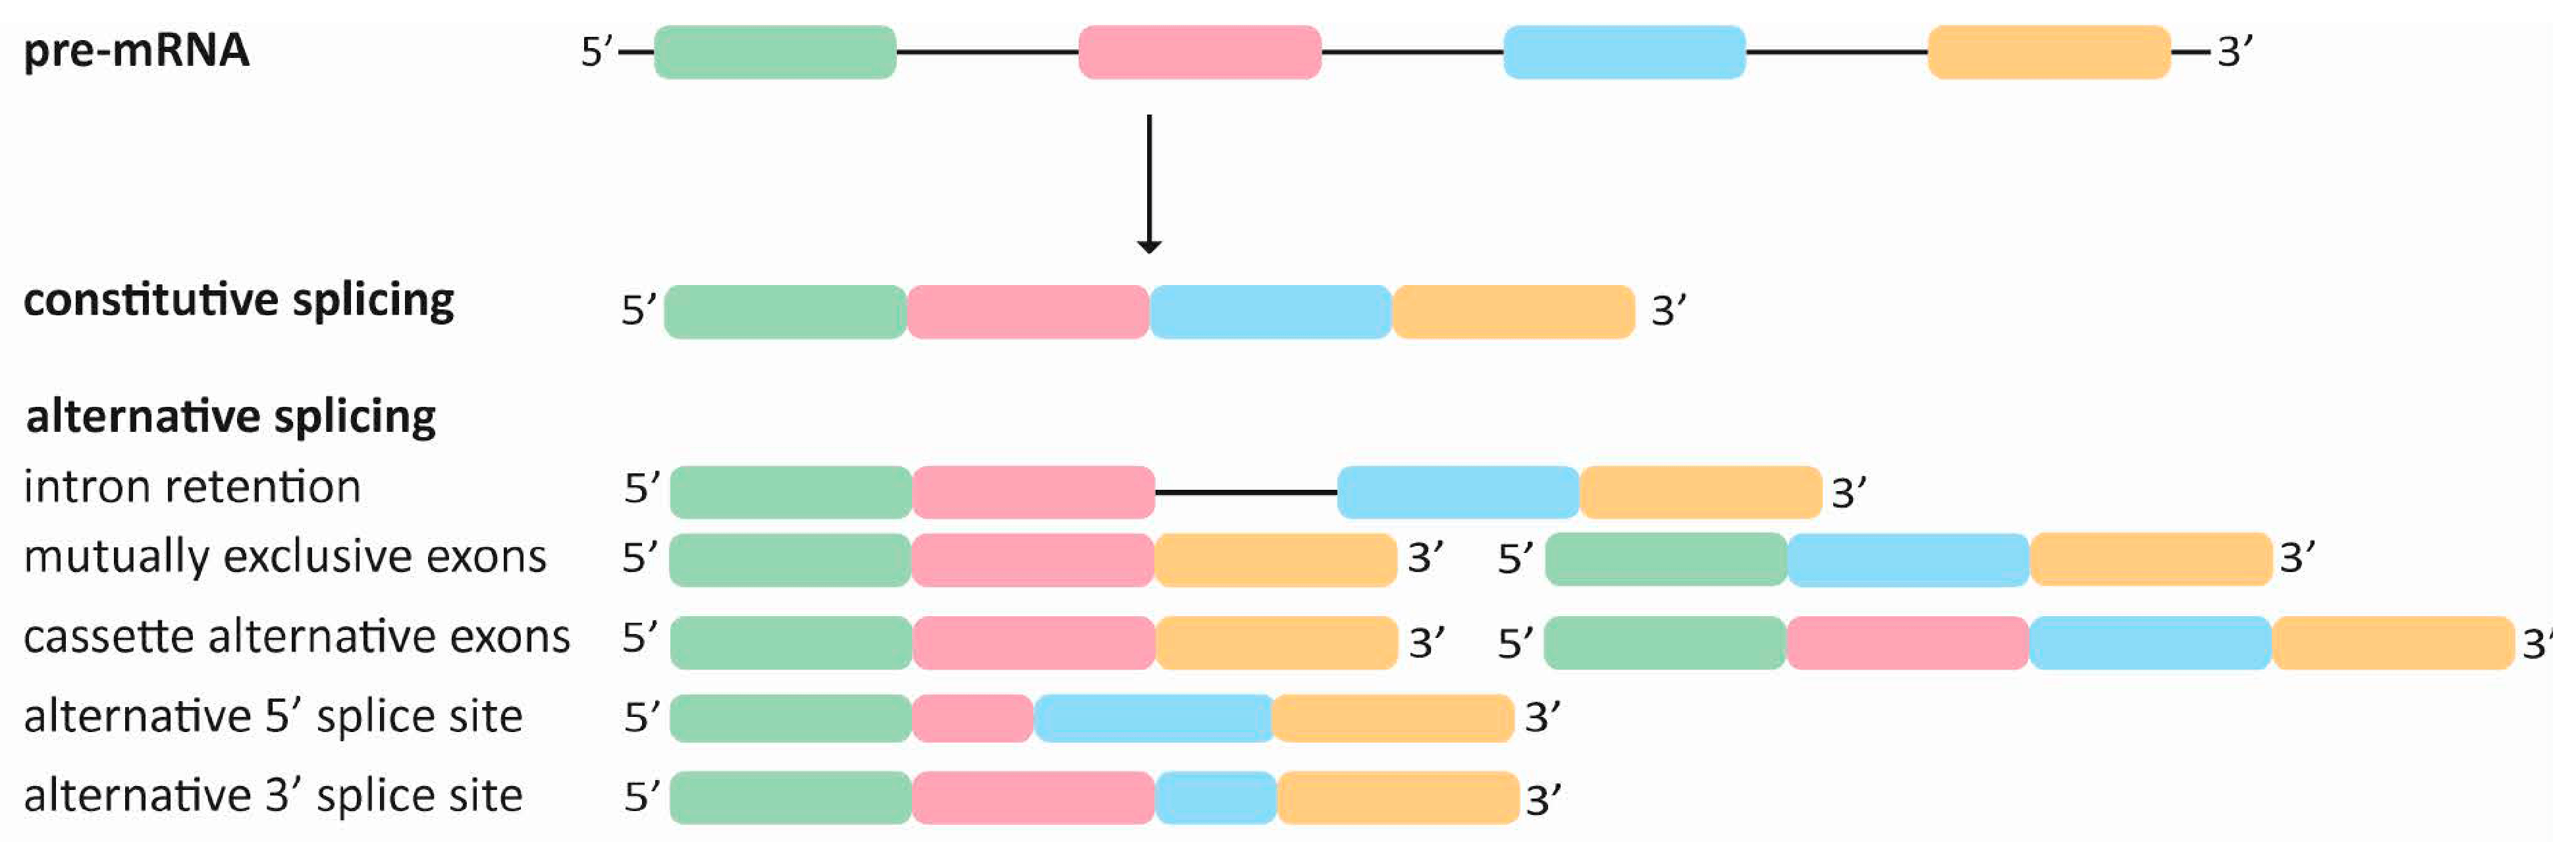
\includegraphics[keepaspectratio, width  = \textwidth]{img/altSplicing}\\ 
	\blfootnote{From: van Haaren et al 2024 - Int. J. Mol. Sci.} 
	
\end{frame}

\begin{frame}
	\frametitle{Gene Regulation}

	\begin{columns}
		\begin{column}{0.5\textwidth}
		\centering	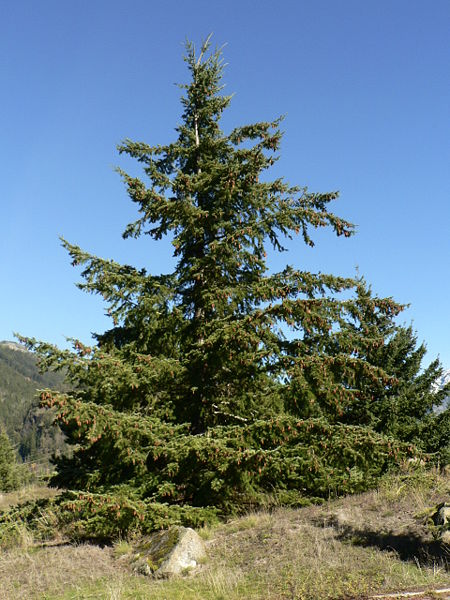
\includegraphics[keepaspectratio, width  = \textwidth]{img/doug-fir}\\ 
	\end{column}
		\begin{column}{0.5\textwidth}
			\begin{itemize}
				\scriptsize

			\item[] Every cell contains the same genes in a multicellular organism,  how do cells know whether to make a pollen or seed cone, a shoot or a root? \pause
			\item[] The \textbf{timing}, \textbf{location} and \textbf{extent} of gene expression are controlled  \pause
			\item[] The set of genes \textbf{expressed} in a cell determines the properties and the functions of the cell \pause
			\item[] In eukaryotes, gene regulation can occur at many steps 
			\end{itemize}
			\end{column}
	
			\end{columns}
	
\end{frame}




\begin{frame}
	
	\Huge
	Questions? \\ \pause
	Let's take a short break
	
\end{frame}


\begin{frame}
	\frametitle{How Do Mutations Influence Phenotypes?}

	\centering	\includegraphics[keepaspectratio, width  = 0.7\textwidth]{img/loganTalking2}\\ \pause
	
	\scriptsize Changes in DNA can potentially influence what proteins do as well as how and when they are regulated \\
	\vspace{10pt}
	Functionally characterising the effects of individual mutations is extremely time-intensive and difficult for an organisms like Douglas-fir
	
	\blfootnote{Logan is right, but genetic variation comes in many forms and these different forms may influence genes and their expression in different ways}
\end{frame}

\begin{frame}
\Large 	How can we locate genomic regions that could potentially influence phenotypes?
\end{frame}


\begin{frame}
	\frametitle{Identifying Genes in DNA Sequences}
		
	\begin{columns}
		\begin{column}{0.5\textwidth}
			
		Two Fundamental Methods
			\begin{itemize}
				\item[--] Search for start/stop codons\textsuperscript{remember the genetic code!}
				\item[--] Sequence RNA and map that to the genome
				\end{itemize}
		\end{column}
		\begin{column}{0.5\textwidth}
						\centering	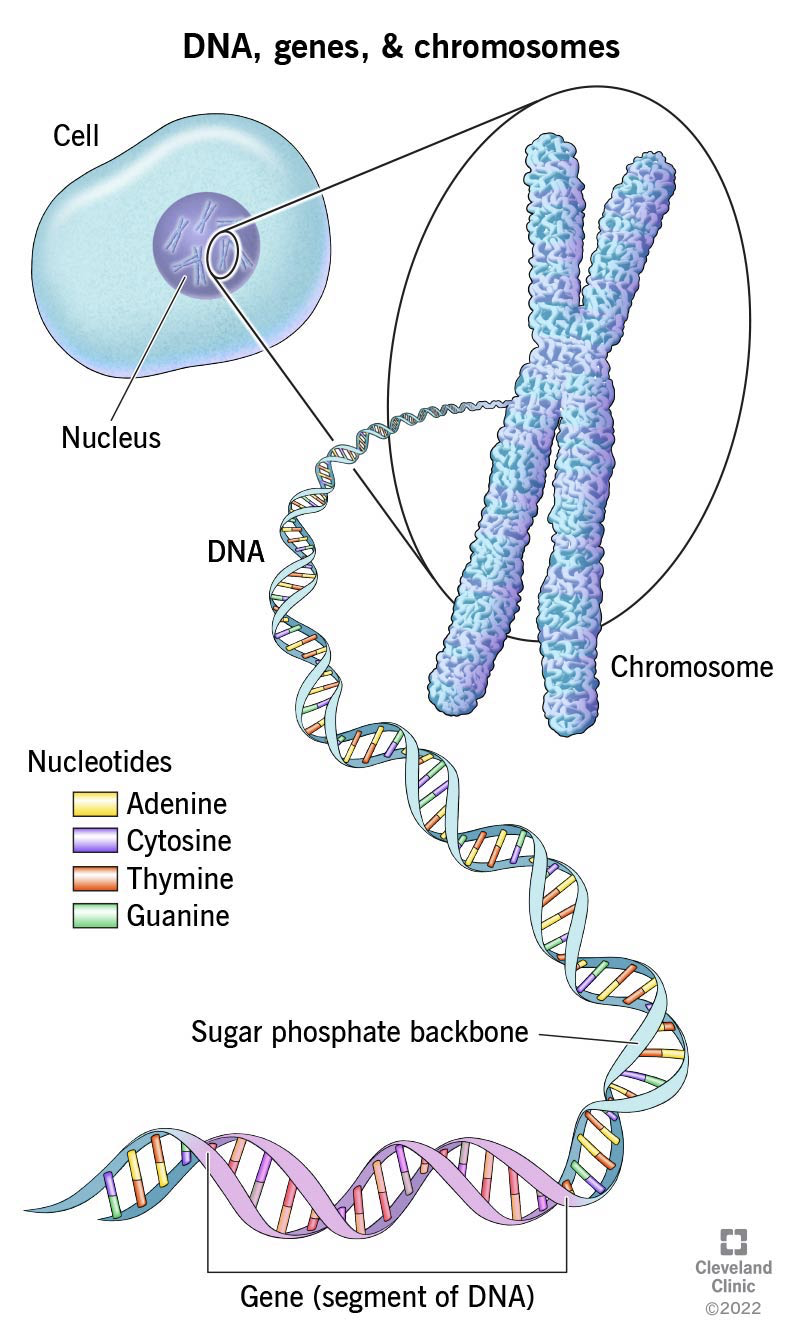
\includegraphics[keepaspectratio, width  = 0.8\textwidth]{img/geneOnDNA}
		\end{column}
	\end{columns}
	
\blfootnote{We refer to the identification of genes in a genome as "annotation"}
\end{frame}


\begin{frame}
	\frametitle{RNA Sequencing - Aligning to Reference Genome}
	\centering	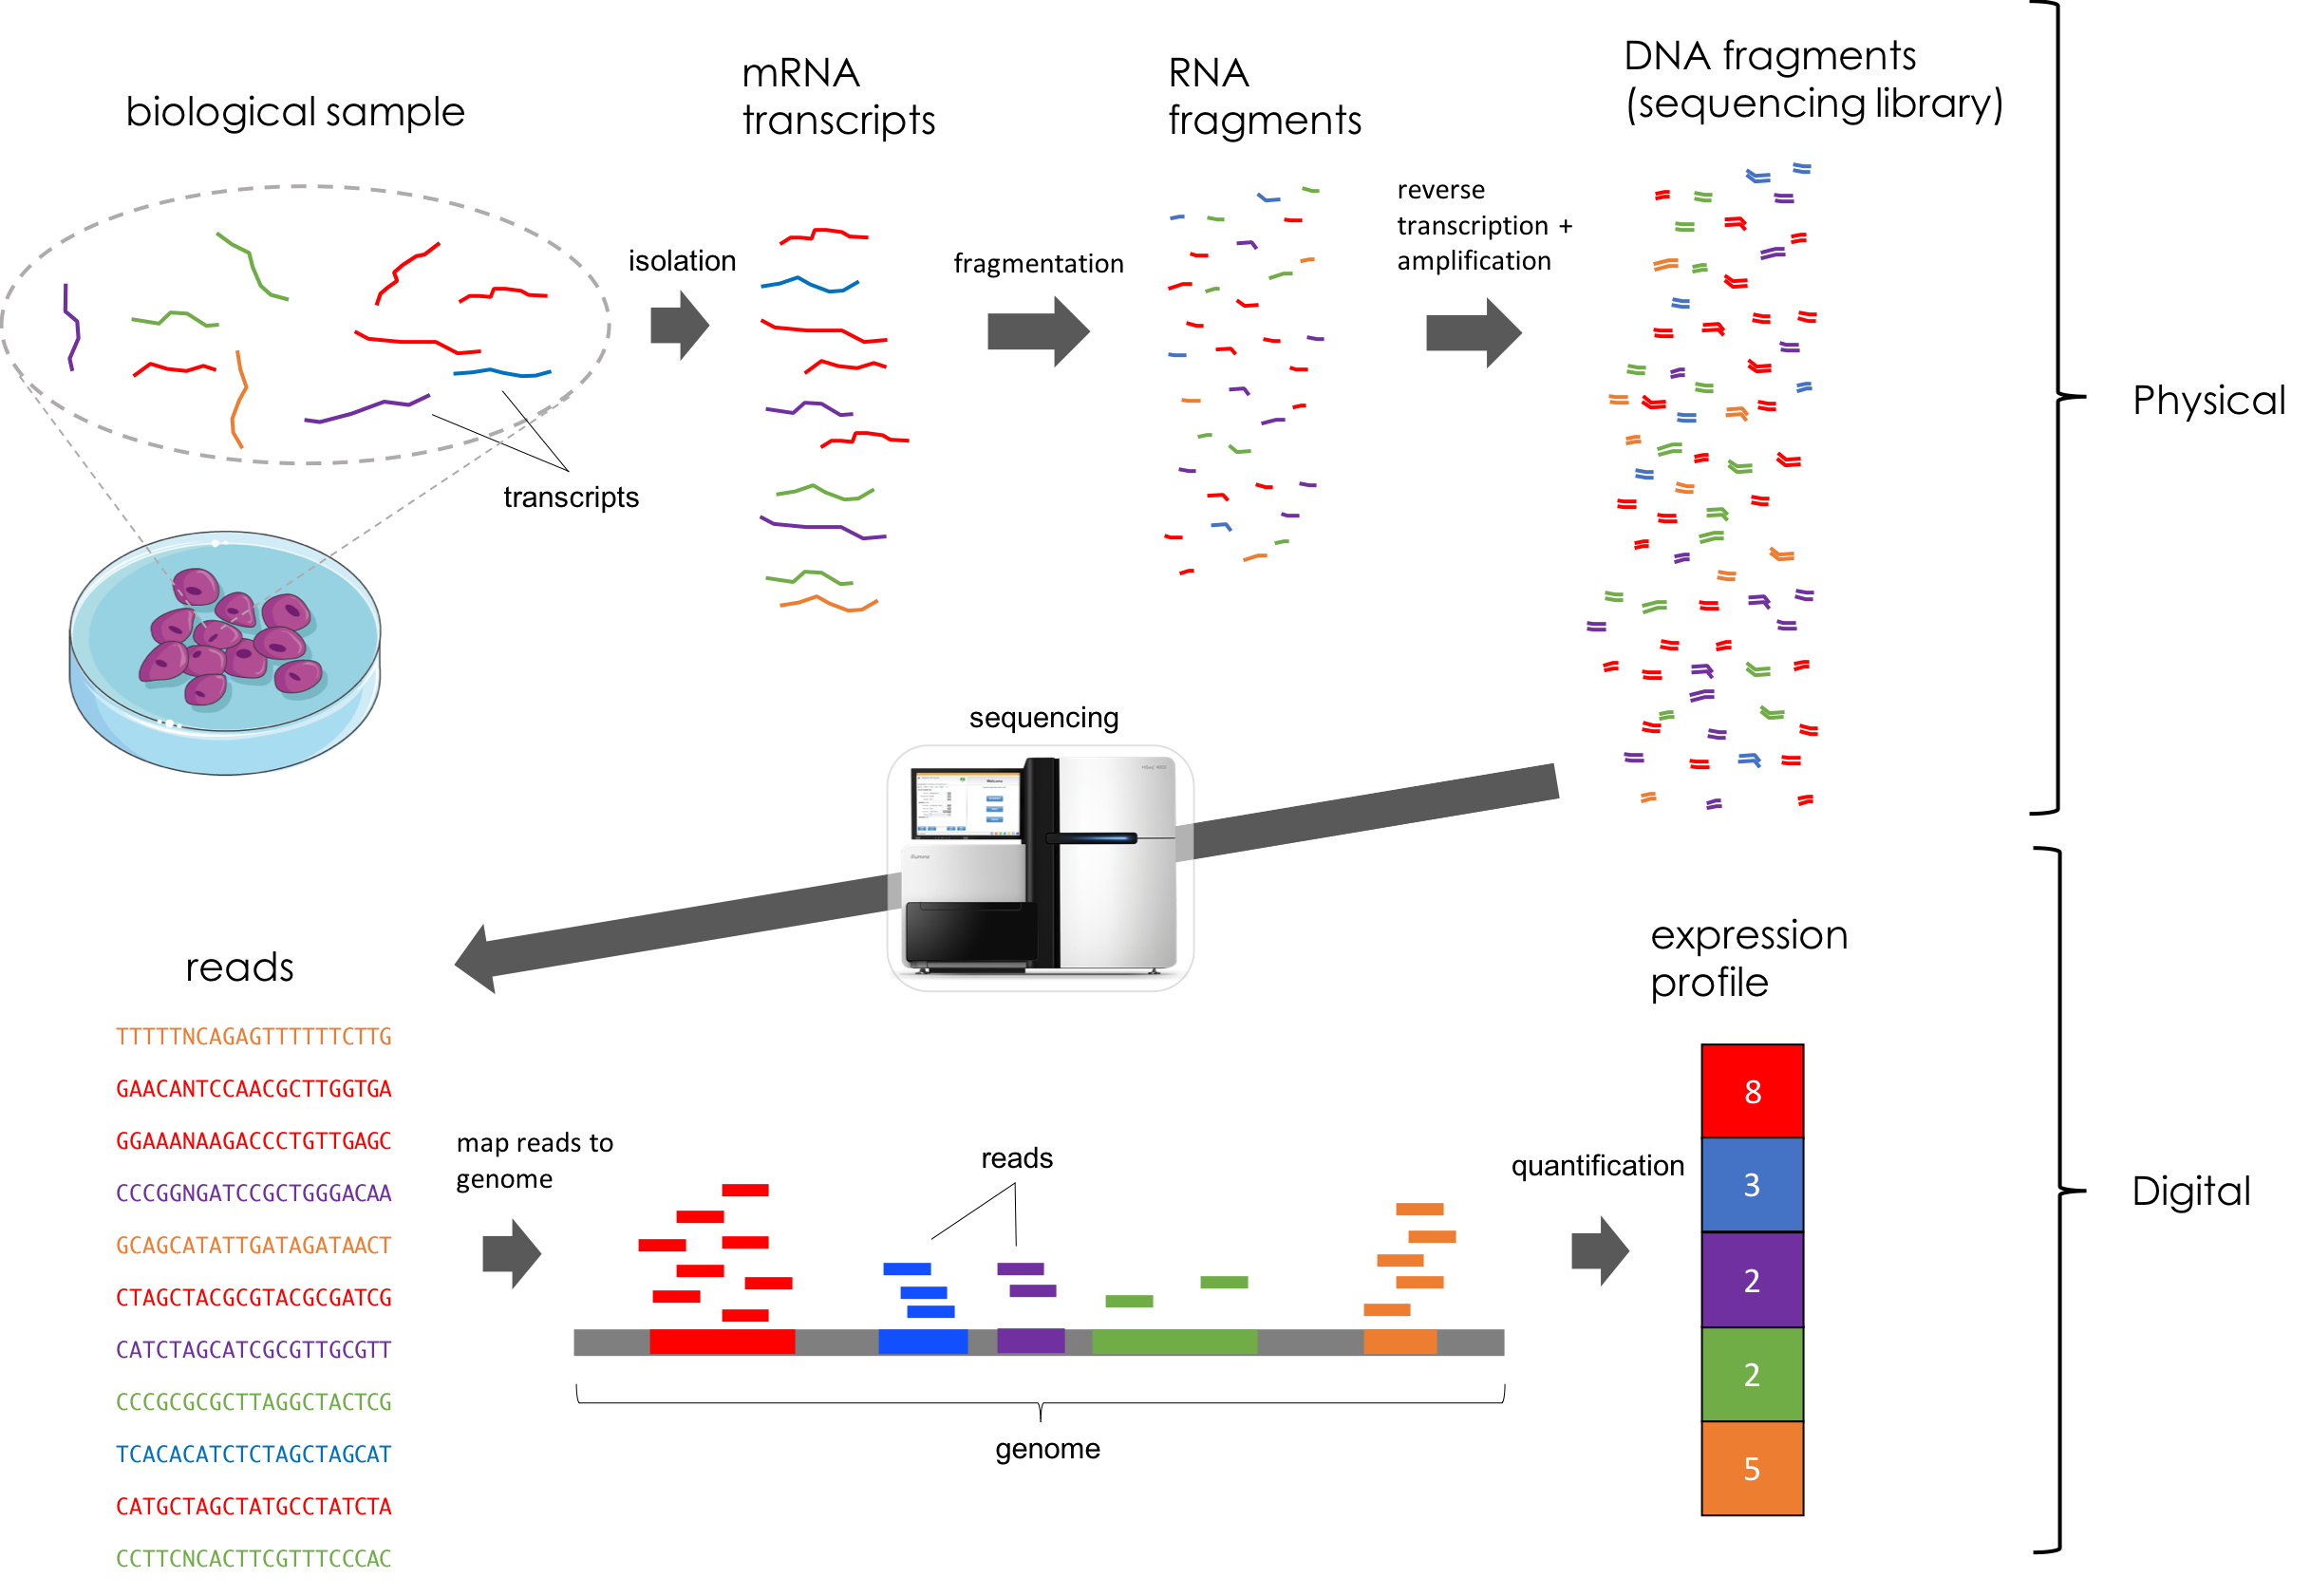
\includegraphics[keepaspectratio, width  = 0.9\textwidth]{img/RNA_seq}
	\blfootnote{Note the use of reverse transcription to convert RNA to DNA!\\ Image from: \url{https://mbernste.github.io/posts/rna_seq_basics/}}
\end{frame}



\begin{frame}
	\frametitle{Central Dogma of Molecular Biology}
	
	
	\centering	\Large \textit{``DNA makes RNA, and RNA makes protein"} \blfootnote{Francis Crick 1957}
	
	\centering	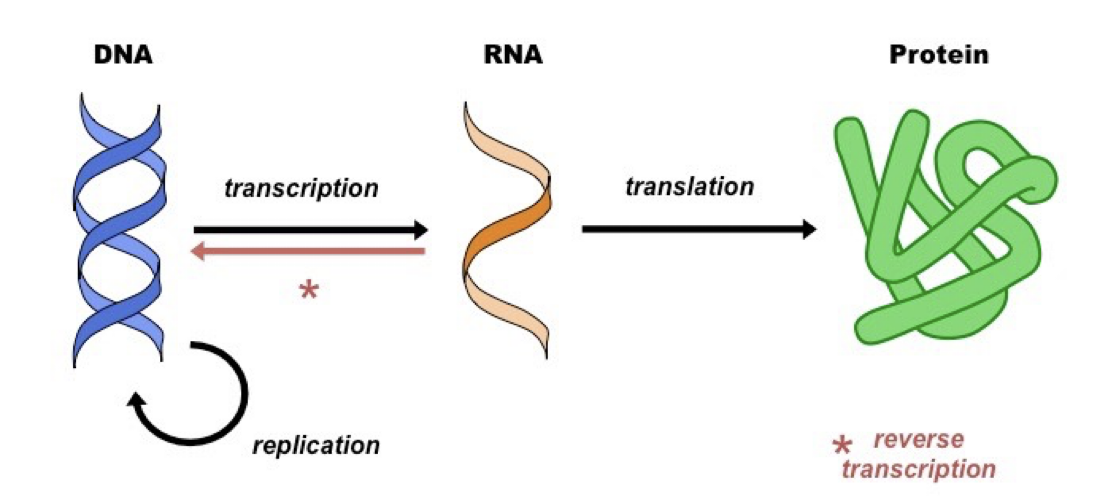
\includegraphics[keepaspectratio, width  = \textwidth]{img/dogma}\\ 
	
	\scriptsize \centering	It means that there is a one-way flow of information \\(\textit{But exceptions abound!})
	
\end{frame}



\begin{frame}
	\frametitle{RNA Sequencing}
	\centering	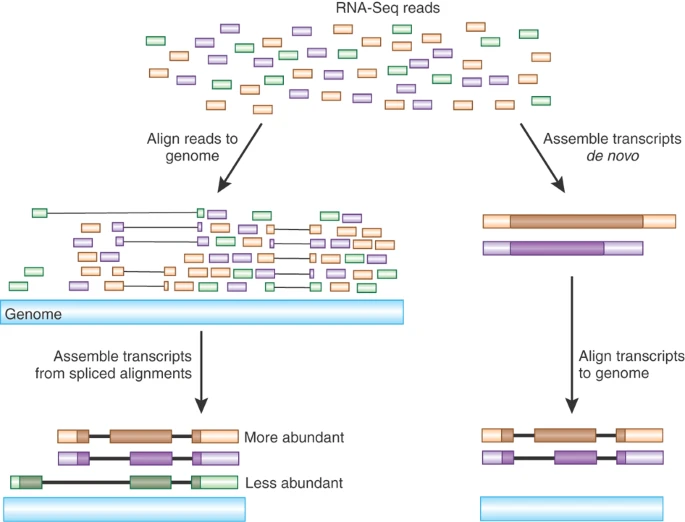
\includegraphics[keepaspectratio, width  = 0.9\textwidth]{img/rnaReadAlignment}
	\blfootnote{Image from: Haas and Zody 2010 \textit{- Nat Biotech.}}
\end{frame}



\begin{frame}
	\frametitle{Douglas-fir Genes}
	\scriptsize
	The following data comes from a recent annotation of the Douglas-fir genome
	\vspace{10pt}

	\begin{columns}
		\begin{column}{0.7\textwidth}
			\begin{tabular}{r|c}
				Total genes	& 51,419\\
				Average gene length (bp) & 17,967.11\\
				Median gene length (bp) & 1,962 \\
				Multiexonics & 41,595\\
				Monoexonics & 9,824\\
				Longest intron (kb) & 778,429\\
				Average number of exons per multiexonic gene& 4.73\\
				
			\end{tabular}		
		\end{column}
		\begin{column}{0.3\textwidth}
			\centering	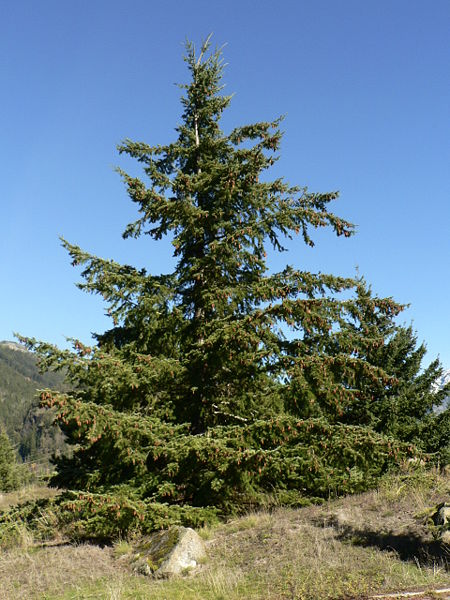
\includegraphics[keepaspectratio, width  = \textwidth]{img/doug-fir}
		\end{column}
	\end{columns} 
	\vspace{10pt}
	$51,419$ genes with an average length of $17,967bp$ that gives us an estimate that $924Mbp$ of the Douglas-fir genome codes for protein\\
	\vspace{10pt}
	That's roughly 5\% of the 16Gbp genome -\textbf{ what's the rest of it doing?}
	\blfootnote{Data from: Velasco et al 2023 - \textit{G3}}
\end{frame}

\begin{frame}
	
	\frametitle{Identifying Gene Regulatory Elements}
\scriptsize	If particular regions have functional roles (e.g. enhancers, promoters etc.) we expect that mutating them would be harmful most of the time\\
	For that reason, we expect that \textbf{functional} regions of non-coding DNA to be conserved through evolutionary time
\pause
				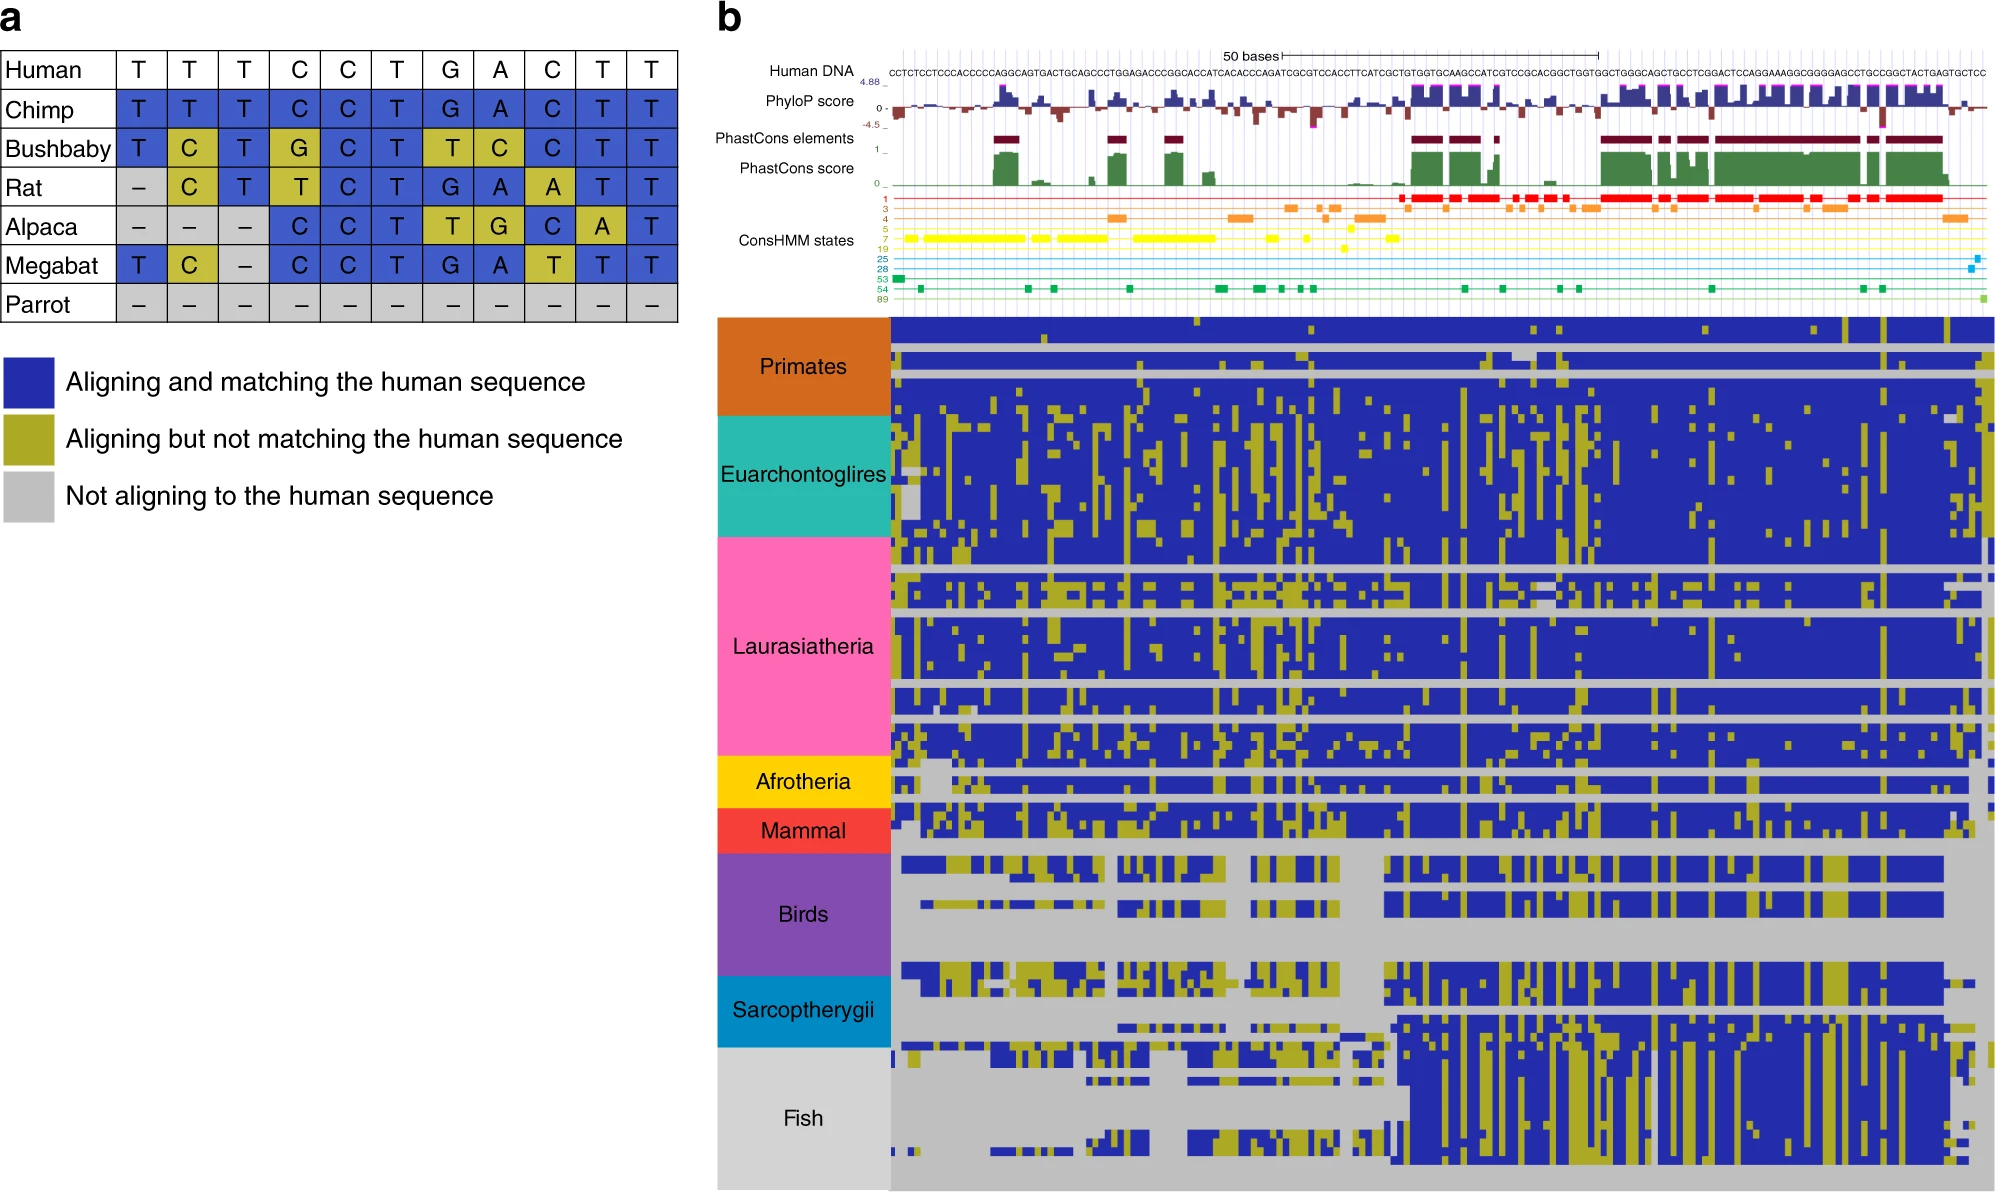
\includegraphics[keepaspectratio, width  = 0.9\textwidth]{img/sequenceConservation}
				
\blfootnote{Conserved non-coding elements identified in this way overlap with regions of accessible chromatin}
\end{frame}

\begin{frame}
	\frametitle{Noncoding ("Junk") DNA}

\begin{columns}
	\begin{column}{0.5\textwidth}
\scriptsize
Noncoding DNA sequences are components of an organism's DNA that do not encode proteins\\
\vspace{10pt}
Noncoding DNA makes up the vast majority of the total DNA in Douglas-fir, the precise fraction varies a lot among species \\
\vspace{10pt}
Beyond genes and gene regulatory elements, tree genomes are filled with stuff:\\
\vspace{10pt}

	\begin{itemize}
		
\item[--]	Some noncoding DNA is transcribed into non-coding RNAs
\item[--] Transposable elements (see last lecture)
\item[--] 	Pseudogenes - the remnants of old genes left in the DNA sequence
\end{itemize}
\end{column}
\begin{column}{0.5\textwidth}
				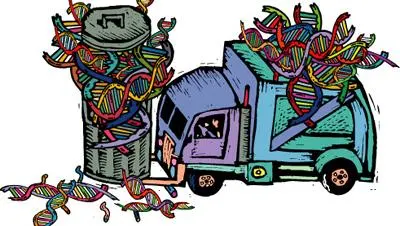
\includegraphics[keepaspectratio, width  = 0.9\textwidth]{img/junk}
\end{column}
\end{columns}
\end{frame}


\begin{frame}
	\frametitle{Learning Outcomes}
	\begin{itemize}
		\item[--] Describe gene structure
		\item[--] The various roles of RNA
		\item[--] Describe gene expression
		\item[--] Identifying functional regions in a genome
		 
	\end{itemize}
\end{frame}

\end{document}




